\chapter{Ensemble canonico}
Se al posto dell'energia interna si controlla la temperatura del sistema, allora l'ensemble che descrive il sistema è l'ensemble canonico. Il principale motivo per usare questo ensemble piuttosto che il microcanonico è semplicemente che la temperatura $T$ è nettamente più semplice da controllare e misurare rispetto all'energia $E$.
\begin{figure}[h]
    \centering
    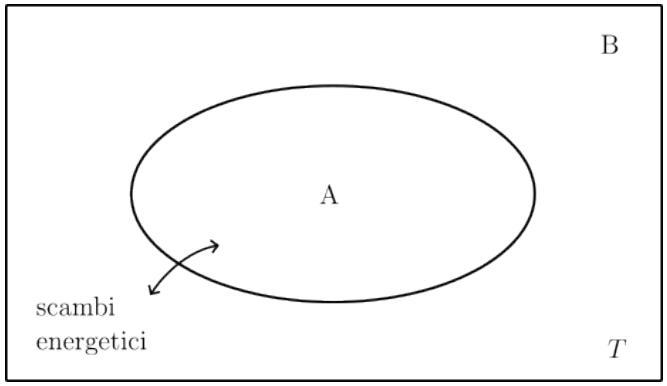
\includegraphics[width=0.45\linewidth]{Immagini/sistema generico (canonico).png}
    \caption{sistema generico per l'ensemble canonico.}
    \label{fig: sistema generico (canonico)}
\end{figure}
Si consideri, in riferimento alla figura \ref{fig: sistema generico (canonico)}, un sottosistema $A$ posto a contatto termico con un termostato $B$, ossia un sistema avente capacità termica molto maggiore di quella di $A$, in modo che quando viene stabilito l'equilibrio termico tra $A$ e $B$ questo avvenga alla temperatura di $B$. Essenzialmente, impostando la temperatura di $B$ si ha la certezza che $A$ prima o poi raggiungere tale temperatura. Sia ora $E$ l'energia totale del sistema, data dalla somma $E = E_A + E_B$. Per il sistema complessivo, nel caso microcanonico, i microstati sono tutti equiprobabili e il loro numero è dato da $\Omega(E)$. Si supponga adesso che $A$ sia in un microstato $\nu$ con energia $E_\nu$, di conseguenza $B$ può trovarsi in un qualsiasi stato purché abbia energia $E - E_\nu$, pertanto il numero di tali microstati è $\Omega_B(E - E_\nu)$. Siccome i microstati sono tutti equiprobabili, la probabilità che il microstato complessivo sia nello stato appena descritto è data da
\begin{equation}
    P(\nu) = \frac{\Omega_B(E - E_\nu)}{\Omega(E)}.
\end{equation}
Quindi, fissando $E_\nu$ risultano accettabili tutti gli stati di $B$ con energia complementare. 
\begin{obs}
    In linea di principio, a causa delle fluttuazioni avere energia alta in $A$, ma con la condizione che quella in $B$ sia bassa, e questo accade in pochi casi; pertanto, questi casi possono essere trascurati e ci si aspetta che la probabilità non sia uguale per tutte le energie.
\end{obs}
Dunque, trascurando $\Omega(E)$ dato che si tratta di una normalizzazione indipendente da $\nu$, si ha
\begin{equation}
    P(\nu) \propto \Omega_B(E - E_\nu) = \exp{[\log{\Omega_B(E - E_\nu)}]}.
\end{equation}
Consistentemente con l'ipotesi che $B$ abbia una capacità termica molto maggiore di quella di $A$, si può assumere che $E \gg E_\nu$, così facendo si può espandere il logaritmo in serie di Taylor ottenendo
\begin{equation}
    \log{\Omega_B(E - E_\nu)} = \log{\Omega_B(E)} - \frac{\p}{\p E}(\log{\Omega_B})E_\nu + \cdots,
\end{equation}
da cui, usando l'entropia di Boltzmann \eqref{eq: entropia (microcanonico)} e l'equazione di stato termica \eqref{eq: equazioni di stato da S}, si ha
\begin{equation}
    \frac{\p}{\p E}(\log{\Omega_B}) = \frac{1}{k}\frac{\p S_B}{\p E} = \frac{1}{kT_B} \equiv \beta_B,
\end{equation}
dove $T_B$ è la temperatura di $B$ che all'equilibrio coincide con quella di $A$. Dunque, la probabilità $P(\nu)$ risulta essere
\begin{equation}
    P(\nu) \propto e^{-\beta E_\nu},
\end{equation}
dove $e^{-\beta E_\nu}$ è tipicamente chiamato ``fattore di Boltzmann''. Ricapitolando, la probabilità che il microstato complessivo sia nello stato in questione è determinata a partire da $B$, ma all'equilibrio, a meno di una costante di normalizzazione, è la stessa del sistema $A$. Introducendo ora la costante di normalizzazione $Z$ in modo che 
\begin{equation}
\label{eq: probabilità microstati (canonico)}
    P(\nu) = \frac{e^{-\beta E_\nu}}{Z},
\end{equation}
dalla normalizzazione di $P(\nu)$ impone che $\nsum_\nu P(\nu) = 1$ segue che
\begin{equation}
\label{eq: funzione di partizione (canonico)}
    Z = \nsum_\nu e^{-\beta E_\nu}.
\end{equation}
In generale, la quantità $Z(T,V,N,\dots)$ è detta ``funzione di partizione'' del sistema ed è proprio la funzione che conferma il fatto che nell'ensemble canonico i microstati non sono più tutti equiprobabili: microstati con energia molto più grande rispetto all'energia termica $kT$ sono esponenzialmente soppressi.

\subsubsection{Fluttuazioni dell'energia}
Si consideri un sistema descrivibile tramite l'ensemble canonico, nel limite termodinamico il sottosistema $A$ ha un energia $E_A$ fissata, a meno di fluttuazioni trascurabili delle energie $E_\nu$ dei singoli microstati, che per consistenza deve corrispondere al valor medio delle energie $E_\nu$ dato da
\begin{equation}
\label{eq: valor medio E (canonico)}
    \begin{split}
        \vmedio{E} = \nsum_\nu P(\nu)E_\nu &= \frac{1}{Z}\nsum_\nu E_\nu e^{-\beta E_\nu} \\
        &= -\frac{1}{Z}\frac{\p}{\p\beta}\nsum_\nu e^{-\beta E_\nu} \\
        &= -\frac{\p}{\p\beta}\log{Z}.
    \end{split}
\end{equation}
Quando le variabili di controllo sono $\{T,V,N\}$, il potenziale termodinamico corretto è l'energia libera di Helmoltz $F$, per cui $Z \equiv Z(T,V,N) = e^{-\beta F(T,V,N)}$, dove si è introdotta
\begin{equation}
    F = -\frac{\log{Z}}{\beta}.
\end{equation}
Tramite $F$ è possibile riscrivere \eqref{eq: valor medio E (canonico)} come
\begin{equation}
    \vmedio{E} = \frac{\p}{\p\beta}(\beta F) = F + \beta\frac{\p F}{\p\beta} = F - T\frac{\p F}{\p T},
\end{equation}
dove si è usata la relazione
\begin{equation}
    \beta\frac{\p}{\p\beta} = \frac{\p}{\p(\log{\beta})} = -\frac{\p}{\p(\log{T})} = -T\frac{\p}{\p T},\quad \beta = \frac{1}{kT}.
\end{equation}
Il fatto che $F$ sia proprio l'energia libera di Helmoltz è confermato ricordando l'equazione di stato \eqref{eq: equazioni di stato da F} relativa all'entropia, da cui si ricava la trasformata di Legendre che lega i due potenziali
\begin{equation}
    F = \vmedio{E} -TS.
\end{equation}
Fino ad ora si sono assunte trascurabili le fluttuazioni rispetto al valore medio nel limite termodinamico, anche se l'energia dei microstati $E_\nu$ non è fissata. L'energia termodinamica è ben definita e non si osservano fluttuazioni spontanee rilevanti nel suo valore; tuttavia, questa affermazione deve seguire automaticamente dalla trattazione canonica. Per vederlo, si definisce la fluttuazione di energia come $\delta E = E - \vmedio{E}$, dove $E$ è il valore dell'energia misurata per il sottosistema $A$, il quale deve risultare nullo, ossia $\delta E = 0$. La quantità rilevante è la varianza $\sigma_E^2$ delle fluttuazioni data da
\begin{equation}
    \sigma^2_E := \bigvmedio{(\delta E)^2} = \vmedio{E^2} - \vmedio{E}^2.
\end{equation}
Dalla \eqref{eq: valor medio E (canonico)}, si deduce che
\begin{equation}
    \vmedio{E^2} = \nsum_\nu P(\nu)E_\nu^2 = \frac{1}{Z}\nsum_\nu E_\nu^2 e^{-\beta E_\nu} = \frac{1}{Z}\frac{\p^2Z}{\p\beta^2},
\end{equation}
considerando quindi la quantità
\begin{equation}
    \frac{\p\vmedio{E}}{\p\beta} = -\frac{\p}{\p\beta}\bigg(\frac{1}{Z}\frac{\p Z}{\p\beta}\bigg) = \frac{1}{Z^2}\bigg(\frac{\p Z}{\p\beta}\bigg)^2 - \frac{1}{Z}\frac{\p^2Z}{\p\beta^2} \equiv \vmedio{E}^2 - \vmedio{E^2},
\end{equation}
si trova che
\begin{equation}
\label{eq: varianza di E (canonico)}
    \sigma_E^2 = - \frac{\p\vmedio{E}}{\p\beta}.
\end{equation}
Dato che $\vmedio{E}$ è una quantità estensiva, mentre $\beta T$ è intensiva, allora $\sigma^2_E$ è anch'essa estensiva; in particolare, si ha
\begin{equation}
    \sigma_E^2 \simeq N,\quad N\to\infty.
\end{equation}
Quindi, le fluttuazioni relative di energia nel limite termodinamico si comportano come
\begin{equation}
\label{eq: andamento fluttuazioni di E (canonico)}
    \frac{\sigma}{\vmedio{E}} \simeq \frac{\sqrt{N}}{N} = \frac{1}{\sqrt{N}}.
\end{equation}
Dunque, l'assunzione che le fluttuazioni di energia siano trascurabili nel limite termodinamico è giustificata dall'andamento \eqref{eq: andamento fluttuazioni di E (canonico)} di queste ultime in funzione di $N$.
\begin{obs}
    Si nota che l'equazione \eqref{eq: varianza di E (canonico)} connette la varianza $\sigma^2_E$ alle funzioni di risposta $c_{V,N}$; infatti
    \begin{equation}
    \label{eq: relazione tra le fluttuazioni di E e cV,N (canonico)}
        \frac{\p\vmedio{E}}{\p\beta} = \frac{\p T}{\p\beta}\frac{\p\vmedio{E}}{\p T} = -kT^2\frac{\p E}{\p T} = -kT^2c_{V,N} = -\sigma_E^2.
    \end{equation}
    Questo è un esempio del ``fluctuation dissipation theorem'', il quale collega le fluttuazioni all'equilibrio con la risposta del sistema alla variazione di parametri di controllo e a fenomeni di dissipazione quando si è fuori equilibrio.
\end{obs}

\subsubsection{Ensemble canonico quantistico}
Nel limite classico spesso i livelli di energia sono continui e tipicamente la somma sui microstati diventa un integrale sullo spazio delle fasi, passando così dal discreto al continuo. Nel contesto quantistico, nella base dell'energia, la matrice densità $\rho$ è diagonale e su di essa sono presenti le probabilità $P(\nu)$ dei singoli microstati, quindi
\begin{equation}
    \rho_{\mu\nu} = P(\nu)\delta_{\mu\nu},\quad P(\nu) = \frac{e^{-\beta E_\nu}}{Z}.
\end{equation}
In una base qualsiasi, l'operatore densità $\hatrho$ è dato da
\begin{equation}
    \hatrho = \frac{e^{-\beta\hatH}}{Z},\quad Z = \Tr{e^{-\beta\hatH}},
\end{equation}
dove $Z$ corrisponde alla normalizzazione per avere $\Tr{\hatrho} = 1$. Pertanto, il valore di aspettazione $\vmedio{\hatO}$ di un'osservabile $O$ rappresentata dal corrispettivo operatore autoaggiunto $\hatO$ è dato dal rapporto
\begin{equation}
    \vmedio{\hatO} = \frac{\Tr{\hatO e^{-\beta\hatH}}}{Z} = \frac{\Tr{\hatO e^{-\beta\hatH}}}{\Tr{e^{-\beta\hatH}}}.
\end{equation}

\section{Entropia di Gibbs}
Fino ad ora si è derivata la forma della probabilità $P(\nu)$ tramite assunzioni ad hoc sia per l'ensemble microcanonico che per il canonico. Tuttavia, esiste una formulazione generale, dovuta a Gibbs, che permette di trovare l'espressione del funzione di entropia per un qualsiasi ensemble
\begin{equation}
\label{eq: definizione entropia Gibbs}
    \SG[P(\nu)] = -k\nsum_\nu P(\nu)\log{P(\nu)} = -k\vmedio{\log{P(\nu)}}.
\end{equation}
In altre parole, è possibile derivare la statistica dell'equilibrio tramite un'espressione generale dell'entropia\footnote{L'espressione \eqref{eq: definizione entropia Gibbs} è supposta valere anche fuori equilibrio.}, data dalla \eqref{eq: definizione entropia Gibbs}, definita come un funzionale delle possibili forme funzionali della probabilità all'equilibrio. Siccome per condizioni esterne fissate l'equilibrio viene raggiunto al massimo dell'entropia, ciò implica che tra le possibili probabilità $P(\nu)$ vengono selezionate proprio quelle che massimizzano l'entropia. Pertanto, si può determinare la probabilità all'equilibrio massimizzando il funzionale \eqref{eq: definizione entropia Gibbs} e tenendo conto degli eventuali vincoli.

Come prima cosa, si deve verificare che l'entropia $\SG$ sia una quantità estensiva. Perciò, si considerano due sottosistemi indipendenti $A$ e $B$, componenti di un sistema complessivo $A\cup B$. La probabilità congiunta, data l'indipendenza di $A$ e $B$, è data da 
\begin{equation}
    P_{AB}(\nu_A,\nu_B) = P_A(\nu_A)P_B(\nu_B).
\end{equation}
Utilizzando adesso le proprietà dei logaritmi e le condizioni di normalizzazione per le probabilità $\nsum_{\nu_A}P_A$ e $\nsum_{\nu_B}P_B$ si ottiene
\begin{equation}
    \begin{split}
        \SG_{AB} &= -k\nsum_{\nu_A}\nsum_{\nu_B}P_{AB}(\nu_A,\nu_B)\log{ P_{AB}(\nu_A,\nu_B)} \\
        &= -k\nsum_{\nu_A}\nsum_{\nu_B}P_A(\nu_A)P_B(\nu_B)[\log{P_A(\nu_A)} + \log{P_B(\nu_B)}] \\
        &=-k\nsum_AP_A(\nu_A)\log{P_A(\nu_A)}\nsum_{\nu_B}P_B(\nu_B) \\
        &-k\nsum_{\nu_B}P_B(\nu_B)\log{P_B(\nu_B)}\nsum_{\nu_A}P_A(\nu_A) \\
        &\equiv \SG_A + \SG_B.
    \end{split}
\end{equation}
Nel limite classico, l'entropia di Gibbs $\SG$ si riduce alla formula di Boltzmann
\begin{equation}
    \SG = -k\sum_{\nu = 1}^\Omega\frac{1}{\Omega}\log{\frac{1}{\Omega}} = k\log{\Omega} \equiv S;
\end{equation}
invece, nel contesto quantistico, $\SG$ si può riscrivere come
\begin{equation}
    \SG[\hatrho] = -k\Tr{\hatrho\log{\hatrho}} = k\SvN,
\end{equation}
che corrisponde, a meno di una costante moltiplicativa, all'entropia di von Neumann \eqref{eq: definizione entropia von Neumann}, connettendo così l'entropia termodinamica alla quantità di informazione contenuta in un sistema quantistico.

\subsubsection{Derivazione di \texorpdfstring{$\bm{P(\nu)}$}{P(nu)} nell'ensemble microcanonico}
Sempre nel limite classico, è possibile derivare la forma di $P(\nu)$ massimizzando il funzionale $\SG[P(\nu)]$ rispetto a $P(\nu)$ tenendo del vincolo $\nsum_\nu P(\nu) = 1$. Per farlo, si utilizza la tecnica dei moltiplicatori di Lagrange, in questo caso si ha
\begin{equation}
    \tilde{\SG}[P] = \SG[P] + \alpha_0\bigg(\nsum_\nu P(\nu) - 1\bigg),
\end{equation}
la cui variazione deve risultare nulla rispetto ad una variazione $\delta P(\nu)$ arbitraria
\begin{equation}
    \begin{split}
        0 \equiv \delta\tilde{\SG}[P] &= \delta\bigg(-k\nsum_\nu P(\nu)\log{P(\nu)} + \alpha_0\nsum_\nu P(\nu)\bigg)  \\
        &= \nsum_\nu\delta P(\nu)\bigg(-k\log{P(\nu)} - k + \alpha_0\bigg),
    \end{split}
\end{equation}
dove essendo la variazione in $P(\nu)$ arbitraria, necessariamente il termine nella parentesi tonda deve annullarsi per soddisfare la condizione di massimizzazione, per cui
\begin{equation}
    P(\nu) = e^{-1 + \alpha_0/k}.
\end{equation}
Imponendo ora il vincolo $\nsum_\nu P(\nu) = 1$ si ottiene
\begin{equation}
    \Omega e^{-1 + \alpha_0/k} = 1\quad\Rightarrow\quad P(\nu) = \Omega^{-1},
\end{equation}
che è esattamente il risultato trovato nella \eqref{eq: probabilità microstati (microcanonico)}.

\subsubsection{Derivazione di \texorpdfstring{$\bm{P(\nu)}$}{P(nu)} nell'ensemble canonico}
Come già detto, nell'ensemble canonico i microstati $\nu$ non hanno tutti la stessa energia, tuttavia all'equilibrio si ha un'energia termodinamica complessiva pari a
\begin{equation}
    E \equiv \vmedio{E} = \nsum_\nu E_\nu P(\nu).
\end{equation}
Si deve fare attenzione che ora si hanno due vincoli, corrispondenti proprio a
\begin{equation}
    \nsum_\nu P(\nu) = 1,\quad \nsum_\nu P(\nu)E_\nu = E.
\end{equation}
Dato il numero di vincoli, sono necessari due moltiplicatori di Lagrange, per cui
\begin{equation}
    \tilde{\SG}[P] = \SG[P] + \alpha_0\bigg(\nsum_\nu P(\nu) - 1\bigg) + \alpha_E\bigg(\nsum_\nu P(\nu)E_\nu - E\bigg).
\end{equation}
In modo analogo a quanto fatto per l'ensemble microcanonico, si massimizza il funzionale di entropia ponendo $\delta\tilde{\SG}[P] = 0$ rispetto ad una $\delta P(\nu)$ arbitraria. Si pone quindi
\begin{equation}
    \begin{split}
        0 \equiv \delta\tilde{\SG}[P] &= \delta\bigg(-k\nsum_\nu P(\nu)\log{P(\nu)} + \alpha_0\nsum_\nu P(\nu) + \alpha_E\nsum_\nu P(\nu)E_\nu\bigg) \\
        &= \nsum_\nu \delta P(\nu)(-k\log{P(\nu)} - k + \alpha_0 + \alpha_E E_\nu),
    \end{split}
\end{equation}
il quale si annulla se e solo se il termine nella parentesi tonda è nullo, per cui si ha
\begin{equation}
    P(\nu) = e^{-1 + \alpha_0/k}e^{\alpha_E E_\nu/k}.
\end{equation}
Imponendo il vincolo di normalizzazione si fissa il moltiplicatore $\alpha_0$
\begin{equation}
    \nsum_\nu P(\nu) = \nsum_\nu e^{-1 + \alpha_0/k}e^{\alpha_E E_\nu/k} = 1\quad\Rightarrow\quad Z = \nsum_\nu e^{\alpha_E E_\nu/k};
\end{equation}
per imporre invece il secondo vincolo, tenendo conto della condizione di normalizzazione $Z = \nsum_\nu e^{\alpha_E E_\nu/k}$ appena trovata, si riscrive l'entropia come
\begin{equation}
    \begin{split}
        \SG = -k\nsum_\nu P(\nu)\log{P(\nu)} &= -k\nsum_\nu P(\nu)\bigg(\frac{\alpha_E}{k}E_\nu - \log{Z}\bigg) \\
        &= -\alpha_E\vmedio{E} + k\log{Z},
    \end{split}
\end{equation}
da cui, confrontandola con l'equazione di stato termica \eqref{eq: equazioni di stato da S} e identificando $E \equiv \vmedio{E}$, segue che
\begin{equation}
    \alpha_E \equiv -\frac{1}{T}.
\end{equation}
Dunque, la probabilità $P(\nu)$ risulta essere
\begin{equation}
    P(\nu) = \frac{e^{-E_\nu/kT}}{Z} = \frac{e^{-\beta E_\nu}}{Z},\quad Z = \nsum_\nu e^{-\beta E_\nu}.
\end{equation}
che coincide proprio con il risultato trovato nella \eqref{eq: probabilità microstati (canonico)}. Tornando infine all'espressione dell'entropia $\SG = \alpha_E\vmedio{E} + k\log{Z}$, sostituendo $\alpha_E = 1/T$ e $\vmedio{E} \equiv E$, si ha
\begin{equation}
    \SG = \frac{E}{T} + k\log{Z}\quad\Rightarrow\quad TS = E + \frac{\log{Z}}{\beta},
\end{equation}
la quale confrontata con $F = E - TS$ restituisce 
\begin{equation}
    F = -\frac{\log{Z}}{\beta}\quad\Rightarrow\quad Z = e^{-\beta F}.
\end{equation}

\section{Legame tra microcanonico e canonico}
Nell'ensemble canonico la termodinamica è derivata a partire dalla funzione di partizione $Z \equiv Z(T,V,N)$ definita dalla \eqref{eq: funzione di partizione (canonico)}, dove tutti i microstati $\nu$ con la medesima energia contribuiscono allo stesso modo. Indicando con $\Omega(E_e,V,N)$ il numero di microstati $\nu_e$ con una data energia $E_e$, si può scrivere
\begin{equation}
    Z(T,V,N) = \nsum_e\sum_{\nu_e = 1}^{\Omega(E_e)} e^{-\beta E_e} = \nsum_e\Omega(E_e)e^{-\beta E_e},
\end{equation}
dove $\Omega(E_e)$ rappresenta la ``degenerazione'' dell'energia $E_e$. Dato che per sistemi macroscopici classici le energie possibili formano un continuo, e che anche per sistemi macroscopici quantistici i livelli sono estremamente densi, è conveniente introdurre un fattore di densità di probabilità $P(E)$ che dipende solo dall'energia. In questo modo, $P(E)dE$ rappresenta la probabilità che il sistema si trovi in un microstato di energia compresa nell'intervallo di energia $(E, E + dE)$. In termini della densità di microstati $g(E)$, definita come
\begin{equation}
\label{eq: definizione g(E) (microcanonico)}
    g(E)\,dE = \Omega(E)|_{\Delta = dE},
\end{equation}
dove $\Omega(E)$ è il numero di microstati in una corona di spessore infinitesimo $dE$ intorno al livello di energia, si ha
\begin{equation}
\label{eq: P(E) in termini di g(E) (canonico)}
    P(E)\,dE = \frac{e^{-\beta E}}{Z}g(E)\,dE,\quad Z(\beta) = \int_0^\infty dE\,g(E)e^{-\beta E}.
\end{equation}
\begin{notz}
    Per semplicità, nel seguito si omette la dipendenza dalle variabili $\{V,N\}$ e si indica la dipendenza dalla temperatura $T$ tramite $\beta$.
\end{notz}
Se si è nel caso in cui $\beta > 0$, come normalmente accade, l'espressione della funzione di partizione nella \eqref{eq: P(E) in termini di g(E) (canonico)} coincide con la trasformata di Laplace della densità di microstati $g(E)$; pertanto, l'equazione può essere invertita ottenendo
\begin{equation}
\label{eq: g(E) in termini di Z(beta) (canonico)}
    g(E) = \frac{1}{2\pi i}\int_\Gamma d\beta\,e^{\beta E}Z(\beta),\quad \beta = \beta_1 + i\beta_2,\,\beta_2 \in \R,\,\Gamma \in \C_\beta,
\end{equation}
dove il cammino di integrazione $\Gamma$ può essere deformato arbitrariamente fintanto che l'integrale converge e non si incontrano singolarità. Per verificare che quest'ultima è effettivamente la formula inversa, si può sostituire la \eqref{eq: P(E) in termini di g(E) (canonico)} nella \eqref{eq: g(E) in termini di Z(beta) (canonico)} ottenendo proprio
\begin{equation}
    \begin{split}
        g(E) &= \frac{1}{2\pi}\int_\R d\beta_2\int_0^\infty dE'\,g(E')e^{-i(\beta_1 + i\beta_2)(E' - E)} \\
        &= \int_0^\infty dE'\,g(E')e^{-\beta_1(E' - E)}\frac{1}{2\pi}\int_\R d\beta_2\,e^{i\beta_2(E' - E)} \\
        &= \int_0^\infty dE'\,g(E')e^{-\beta_1(E' - E)}\delta(E' - E) \\
        &\equiv g(E),
    \end{split}
\end{equation}
dove si è sfruttato il fattore $e^{-\beta_1 E'}$ per invertire l'ordine di integrazione. Quindi, tornando alla \eqref{eq: P(E) in termini di g(E) (canonico)}, nel limite termodinamico si ha
\begin{equation}
\label{eq: definizione g(E) limite TD (microcanonico)}
    g(E)\,dE = \Omega(E)|_\Delta = e^{S(E)/k} \simeq \Omega(E)|_\Delta = g(E) \Delta,\quad \forall\Delta \ll E,
\end{equation}
dove appunto la scelta di $\Delta$ è irrilevante in quanto quantità non estensiva; mentre, il membro di sinistra nel limite termodinamico è
\begin{equation}
    Z(\beta) = e^{-\beta F(\beta)},
\end{equation}
dove $S(E)$ e $F(T)$ sono proprio l'entropia e l'energia libera di Helmholtz, espresse rispettivamente tramite l'ensemble microcanonico e canonico. L'espressione \eqref{eq: P(E) in termini di g(E) (canonico)}, nel limite termodinamico, diventa
\begin{equation}
\label{eq: P(E) in termini di g(E) limite TD (canonico)}
    e^{-F(\beta)/kT} = \frac{1}{\Delta}\int_0^\infty dE\, e^{(S - E/T)/k} \equiv \frac{1}{\Delta}\int_0^\infty dE\, e^{-f(E)},
\end{equation}
dove $E$ non è l'energia termodinamica ma una generica variabile di integrazione. Tuttavia, l'integrale a secondo membro può essere valutato con il metodo del ``punto a sella''. Il massimo dell'esponente si ha per 
\begin{equation}
    \frac{\p f}{\p E} = \frac{\p}{\p E}\bigg(-S + \frac{E}{T}\bigg) = 0\quad\Longleftrightarrow\quad \frac{\p S}{\p E} = \frac{1}{T},
\end{equation}
ossia quando l'energia $E$ coincide proprio con l'energia termodinamica $\vmedio{E}$ del sistema canonico a temperatura $T$. Quindi, il valore medio $\vmedio{E}$ rappresenta anche il valore di $E$ che massimizza la densità di probabilità $P(E)$, ossia il ``valore più probabile''. Tornando all'integrale, questo può essere valutato tramite la formula
\begin{equation}
    \begin{split}
        \frac{1}{\Delta} \int_{0}^{\infty} dE \, e^{-f(E)} &= e^{-f(\langle E \rangle)}\bigg( \frac{1}{\Delta} \sqrt{\frac{2\pi}{f''(\langle E \rangle)}} + \cdots \bigg) \\
        &= \exp\bigg[{-f(\langle E \rangle) - \frac{1}{2} \log \frac{\Delta^2 f''(\langle E \rangle)}{2\pi}} + \cdots\bigg],
    \end{split}
\end{equation}
dato che $f(E)$ è estensiva e scala con $N$, e $f''(E)$ scala con $1/N$. Quindi, il secondo termine nell'esponenziale scala con $\log{N}$ ed è pertanto trascurabile rispetto al primo termine. Il risultato è che l'espressione \eqref{eq: P(E) in termini di g(E) limite TD (canonico)} si riduce a
\begin{equation}
    e^{-F/kT} = e^{[S(\vmedio{E}) - \vmedio{E}/T]/k},
\end{equation}
da cui si ricava nuovamente la trasformata di Legendre che lega $F$ a $\vmedio{E}$ tramite
\begin{equation}
    F = \vmedio{E} - TS.
\end{equation}
Dunque, tale trasformata di Legendre è l'approssimazione termodinamica alla trasformata di Laplace \eqref{eq: P(E) in termini di g(E) (canonico)} che lega la funzione di partizione $Z(\beta)$ alla densità di microstati $g(E)$.

\subsubsection{Trattamento canonico di sistemi non interagenti}
Si consideri un sistema composto di $N$ componenti distinguibili e non interagenti. Un microstato $\nu$ del sistema complessivo corrisponde ad una collezione di microstati $\nu_i$, con $i = 1,\dots,N$, dei vari componenti. L'energia del microstato $\nu$, data l'assenza di interazioni è
\begin{equation}
\label{eq: energia sistema non interagente (canonico)}
    E_\nu = \nsum_iE_{\nu_i}.
\end{equation}
Di conseguenza, la funzione di partizione si fattorizza in quelle di ciascun componente
\begin{equation}
\label{eq: funzione di partizione sistemi non interagenti (canonico)}
    \begin{split}
        Z = \nsum_\nu e^{-\beta E_\nu} &= \nsum_{\nu_1}\cdots\nsum_{\nu_N}e^{-\beta(E_{\nu_1} + \cdots E_{\nu_N})} \\
        &= \nsum_{\nu_1}e^{-\beta E_{\nu_1}}\cdots \nsum_{\nu_N}e^{-\beta E_{\nu_N}} \\
        &= \nprod_iZ_{(i)}.
    \end{split}
\end{equation}
\begin{obs}
    I sistemi reali sono ovviamente sempre interagenti, tuttavia l'approssimazione non interagente può essere valida per i gas in regimi di bassa densità.
\end{obs}
Essendo i componenti identici, secondo la Meccanica quantistica sono anche indistinguibili e la necessità di simmetrizzazione, o antisimmetrizzazione, rispetto ai loro scambi introduce una sorta di interazione statistica. Nei casi più semplici, la conseguenza pratica è l'introduzione di un fattore $1/N!$ per evitare il conteggio di configurazioni che possono essere distinte solo per permutazioni di componenti; in verità, la statistica deve essere imposta tramite il formalismo della matrice densità. Ad ogni modo, la fattorizzazione di $Z$ implica che l'energia libera è anch'essa fattorizzabile
\begin{equation}
    F = -\frac{\log{Z}}{\beta} = -\frac{1}{\beta}\log{\nprod_iZ_{(i)}} = \nsum_i-\frac{1}{\beta}\log{Z_{(i)}} \equiv \nsum_i F_{(i)}.
\end{equation}
Dunque, per sistemi dove è lecito trascurare le interazioni tra le componenti, l'ensemble canonico è estremamente conveniente.

\section{Gas ideale nell'ensemble canonico}
Si consideri un gas ideale monoatomico le cui componenti non hanno gradi di libertà interni, la sua hamiltoniana è
\begin{equation}
    H(q,p) = \sum_{i = 1}^N\frac{|p_i|^2}{2m}.
\end{equation}
Un generico microstato $\nu$ è un punto nello spazio delle fasi $6N$-dimensionale ed è composto dalla collezione di $N$ coordinate $(\vq^i,\vp_i)$ di singola particella. Quindi, valgono le relazioni \eqref{eq: energia sistema non interagente (canonico)} e \eqref{eq: funzione di partizione sistemi non interagenti (canonico)} dove, per evitare il paradosso di Gibbs, si deve introdurre il fattore di Gibbs
\begin{equation}
    Z = \frac{1}{N!}\nprod_iZ_{(i)} = \frac{[Z_{(1)}]^N}{N!},
\end{equation}
dove si è tenuto conto del fatto che la funzione di partizione è la medesima per ogni particella. Proprio per questo motivo, è sufficiente calcolare la funzione di partizione per singola particella
\begin{equation}
    Z_{(1)} = \int\frac{d^3q\,d^3p}{h^3}e^{-\beta H_{(1)}} = \int\frac{d^3q\,d^3p}{h^3}e^{-\beta|\vp|^2/2m}.
\end{equation}
Siccome l'energia non dipende dalle coordinate $\vq$, l'integrale rispetto a $d^3q$ restituisce semplicemente il volume $V$ nello spazio delle coordinate, mentre l'integrale rispetto a $d^3p$ è gaussiano in tre dimensioni; in definitiva, si ha
\begin{equation}
\label{eq: funzione di partizione singola particella (canonico)}
    Z_{(1)} = \frac{V}{h^3}\bigg(\frac{2\pi m}{\beta}\bigg)^{3/2} = V\bigg(\frac{\sqrt{2\pi mkT}}{h}\bigg)^3 \equiv \frac{V}{\lambda_T^3} \equiv \frac{V}{V_T},\quad \lambda_T = \frac{h}{\sqrt{2\pi mkT}},
\end{equation}
dove $\lambda_T$ è detta ``lunghezza d'onda termica'', il cui cubo rappresenta il ``volume termico'' $V_T$. A meno di un fattore $1/\sqrt{\pi}$, $\lambda_T$ corrisponde alla lunghezza d'onda di de Broglie di una particella libera di massa $m$ ed energia pari a $kT$, per la quale $p = \sqrt{2mkT}$. L'espressione \eqref{eq: funzione di partizione singola particella (canonico)} si può interpretare immaginando che alla temperatura $T$ la particella occupi il volume $V_T = \lambda_T^3$ e la funzione di partizione $Z_{(1)}$ conta il volume a disposizione in unità di $V_T$. Sostituendo la \eqref{eq: funzione di partizione singola particella (canonico)} nella \eqref{eq: funzione di partizione sistemi non interagenti (canonico)} si ottiene
\begin{equation}
\label{eq: funzione di partizione gas ideale (canonico)}
    Z = \frac{1}{N!}\bigg(\frac{V}{V_T}\bigg)^N.
\end{equation}
Da questa si può direttamente derivare la termodinamica del sistema; prima di tutto, l'energia libera è data da 
\begin{equation}
    F = -\frac{\log{Z}}{\beta} = -kT\bigg(N\log{\frac{V}{V_T}} - \log{N!}\bigg),
\end{equation}
la quale nel limite termodinamico, usando l'approssimazione di Stirling per il logaritmo \eqref{eq: approssimazione stirling}, si riduce a
\begin{equation}
    F = -NkT\log{\frac{V}{NV_T}} - NkT.
\end{equation}
L'energia interna $E$ di conseguenza è
\begin{equation}
    \begin{split}
        E \equiv \vmedio{E} = -\frac{\p}{\p\beta}\log{Z} &= -\frac{\p}{\p\beta}\bigg(N\log{\frac{V}{V_T}} - \log{N!}\bigg) \\
        &= N\frac{\p}{\p\beta}\log{\beta^{3/2}} \\
        &= \frac{3}{2}NkT,
    \end{split}
\end{equation}
ritrovando l'equazione di stato termica. L'equazione di stato meccanica invece, ricordando l'equazione di stato per la pressione $p$ da \eqref{eq: equazioni di stato da F}, si ricava come
\begin{equation}
    p = \frac{\p}{\p V}\bigg(NkT\log{\frac{V}{NV_T}} + NkT\bigg)\bigg|_{T,N} = \frac{NkT}{V}\quad\Rightarrow\quad pV = NkT.
\end{equation}

\subsection{Trasformata di Laplace per il gas ideale}
Tramite il gas ideale è possibile illustrare la trasformata di Laplace che lega l'ensemble canonico con quello microcanonico, in particolare alle equazioni \eqref{eq: P(E) in termini di g(E) (canonico)} e  \eqref{eq: g(E) in termini di Z(beta) (canonico)}. Ad esempio, dalla funzione di partizione canonica \eqref{eq: funzione di partizione gas ideale (canonico)} si può ottenere la densità di microstati $g(E)$ con la \eqref{eq: P(E) in termini di g(E) (canonico)} come
\begin{equation}
\label{eq: densità di microstati (canonico)}
    \begin{split}
        g(E) &= \frac{1}{2\pi i}\int_\Gamma d\beta\,e^{\beta E}Z(\beta) \\
        &= \frac{1}{N!}\bigg[\frac{V(2m\pi)^{3/2}}{h^3}\bigg]^N\frac{1}{2\pi i}\int_\Gamma d\beta\,e^{\beta E}\beta^{-3N/2} \\
        &\equiv \frac{1}{N!}\bigg[\frac{V(2m\pi)^{3/2}}{h^3}\bigg]^N I_N.
    \end{split}
\end{equation}
L'obiettivo ora è valutare l'integrale 
\begin{equation}
\label{eq: integrale IN (canonico)}
    I_N \equiv \frac{1}{2\pi i}\int_\Gamma d\beta\,e^{\beta E}\beta^{-3N/2},
\end{equation}
ma per farlo si devono distinguere due casi in funzione del valore di $E$.
\begin{caso}[$E < 0$]
    In questo caso, il fattore di convergenza $e^{\beta E}$ consente di applicare il teorema di Jordan e completare il cammino di integrazione $\Gamma$ a destra passando così $\tilde{\Gamma}$, come mostrato in figura \ref{fig: integrale Jordan (TL gas ideale)}. Dato che la funzione $e^{\beta E}\beta^{-3N/2}$ non presenta alcuna singolarità all'interno del cammino $\tilde{\Gamma}$, l'integrale è nullo; in breve
    \begin{equation}
    \label{eq: integrale IN per E < 0}
        I_N = 0,\quad E < 0.
    \end{equation}
\end{caso}
\begin{caso}[$E > 0$]
    In questo caso, il fattore di convergenza $e^{\beta E}$ consente di completare di integrazione a sinistra. Tuttavia, adesso il cammino include delle singolarità e pertanto è necessario distinguere ulteriori due casi:
    \begin{enumerate}
        \item se $N = 2k$ è pari, allora la funzione integranda $\beta^{-3k}$ presenta un polo in $\beta = 0$, mostrato in figura \ref{fig: integrale Jordan (TL E > 0, N pari)}, per cui si ha
        \begin{equation}
        \label{eq: integrale IN per N pari (canonico)}
            \begin{split}
                I_{2k} = \frac{1}{2\pi i}\int_{\tilde{\Gamma}} d\beta\,e^{\beta E}\beta^{-3k} &= \Res{(e^{\beta E}\beta^{-3k})} \\
                &=\Res{\bigg(\sum_{p=0}^\infty\frac{E^p}{p!}\beta^{p-3k}\bigg)} \\
                &= \frac{E^{3N/2 - 1}}{(3N/2 - 1)!} \\
                &= \frac{E^{3N/2 - 1}}{\Gamma(3N/2)},
            \end{split}
        \end{equation}
        dove si è considerato che l'unico termine della serie esponenziale che contribuisce è per $p = 3k - 1$.
        \begin{figure}[h]
            \centering
            \includegraphics[width=0.4\linewidth]{Immagini/integrale Jordan (TL E < 0).png}
            \caption{lemma di Jordan per il calcolo di $I_N$ nel caso $E < 0$.}
            \label{fig: integrale Jordan (TL gas ideale)}
        \end{figure}
        \item se $N = 2k + 1$ è dispari, allora la funzione integranda $\beta^{-3k - 1/2}$ presenta un taglio, per cui si ha
        \begin{equation}
            \begin{split}
                I_{2k+1} &= \frac{1}{2\pi i}\int_{\tilde{\Gamma}}d\beta\,e^{\beta E}\beta^{-3k - 1/2} \\
                &= \frac{1}{2\pi i}\bigg[\int_{-\infty}^0 d\beta_-\,e^{\beta_- E}\beta_-^{-3k - 1/2} + \int_0^{\infty} d\beta_+\,e^{\beta_+ E}\beta_+^{-3k - 1/2} \bigg],
            \end{split}
        \end{equation}
        dove $\beta_+ = e^{i\pi}b$ e $\beta_- = e^{-i\pi}b$, con $b \in \R^+$, sono i valori di $\beta$ sopra e sotto il taglio rispettivamente, come mostrato in figura \ref{fig: integrale Jordan (TL E > 0, N dispari)}, quindi
        \begin{equation}
        \label{eq: integrale IN per N dispari (canonico)}
            \begin{split}
                I_{2k+1} &= -\frac{1}{2\pi i}\int_{-\infty}^0 db\,e^{-bE}(e^{-i\pi})^{-3k}(e^{-i\pi})^{-1/2}b^{-3k - 1/2} \\
                &-\frac{1}{2\pi i}\int_0^\infty db\, e^{-bE}(e^{i\pi})^{-3k}(e^{i\pi})^{-1/2}b^{-3k - 1/2} \\
                &= \frac{1}{2\pi i}2i(-1)^k\int_0^\infty db\,e^{-bE}b^{-3k - 1/2} \\
                &= \frac{(-1)^k}{\pi}\int_0^\infty\frac{dw}{E}e^{-w}\bigg(\frac{w}{E}\bigg)^{-3k - 1/2} \\
                &=\frac{(-1)^k}{\pi} E^{3k + 1/2 - 1}\Gamma(1 - 3k - 1/2) \\
                &= \frac{E^{3k + 1/2 - 1}}{\Gamma(3N/2)},
            \end{split}
        \end{equation}
        dove si è cambiata la variabile in $w = bE$ e dove si è usata la formula di riflessione per la funzione Gamma di Eulero 
        \begin{equation}
            \Gamma\bigg(\frac{3N}{2}\bigg)\Gamma\bigg(1 - \frac{3N}{2}\bigg) = \frac{\pi}{\sin{(3N\pi/2)}} = \frac{\pi}{\sin{[\pi(3k + 1/2)]}} = (-1)^k\pi.
        \end{equation}
    \end{enumerate}
    \begin{figure}[h]
        \centering
        \includegraphics[width=0.55\linewidth]{Immagini/integrale Jordan (TL E > 0, N pari).png}
        \caption{lemma di Jordan per il calcolo di $I_N$ nel caso $E > 0$ con $N$ pari.}
        \label{fig: integrale Jordan (TL E > 0, N pari)}
    \end{figure}
    \begin{figure}[h]
        \centering
        \includegraphics[width=0.55\linewidth]{Immagini/integrale Jordan (TL E > 0, N dispari).png}
        \caption{lemma di Jordan per il calcolo di $I_N$ nel caso $E > 0$ con $N$ dispari.}
        \label{fig: integrale Jordan (TL E > 0, N dispari)}
    \end{figure}
\end{caso}
Dunque, mettendo insieme i risultati ottenuti in \eqref{eq: integrale IN per E < 0}, in \eqref{eq: integrale IN per N pari (canonico)} e nella \eqref{eq: integrale IN per N dispari (canonico)}, l'integrale \eqref{eq: integrale IN (canonico)} vale
\begin{equation}
\label{eq: valore integrale IN}
    I_N = 
    \begin{cases}
        0,\quad E < 0 \\[2ex]
        \dfrac{E^{3N/2 - 1}}{\Gamma(3N/2)},\quad E > 0
    \end{cases}.
\end{equation}
Sostituendo la valutazione di $I_N$ \eqref{eq: valore integrale IN} nella \eqref{eq: densità di microstati (canonico)} si ottiene
\begin{equation}
    g(E) = 
    \begin{cases}
        0,\quad E < 0 \\
        \dfrac{1}{N!}\bigg[\dfrac{V(2\pi mE)^{3/2}}{h^3}\bigg]^N\dfrac{1}{\Gamma(3N/2)E},\quad E > 0
    \end{cases},
\end{equation}
la quale coincide esattamente con quanto ricavato nell'ensemble microcanonico, tramite la \eqref{eq: definizione g(E) (microcanonico)}, nella \eqref{eq: microstati complessivi gas ideale (microcanonico)}.

\subsubsection{Legame con la distribuzione di Maxwell-Boltzmann}
La densità di probabilità di osservare $N$ particelle del sistema con coordinate $\vq\in[\vq^i,\vq^i + d\vq^i]$ e $\vp\in[\vp_i,\vp_i +d\vp_i]$ è data da
\begin{equation}
    \rho(1,\dots,N)d\mu_1\cdots d\mu_N = \frac{1}{N!Z}e^{-\beta H(1,\dots,N)},
\end{equation}
dove la funzione di partizione è
\begin{equation}
     Z = \frac{1}{N!}\int d\mu_1\cdots d\mu_N\,e^{-\beta H(1,\dots,N)},
\end{equation}
e la densità di probabilità è normalizzata secondo
\begin{equation}
    \quad \int d\mu_1\cdots d\mu_N\,\rho(1,\dots,N) = 1.
\end{equation}
Come visto in precedenza, nel caso del gas ideale si hanno
\begin{equation}
    H(1,\dots,N) = \nsum_i\frac{|\vp_i|^2}{2m},\quad Z = \frac{1}{N!}\nprod_i Z_{(i)},
\end{equation}
dove la funzione di partizione di singola particella è indipendente da $i$ ed è data da
\begin{equation}
    Z_{(i)} = \int d\mu_i\,e^{-\beta|\vp_i|^2/2m} = \frac{V}{V_T},\quad \forall i.
\end{equation}
Come accade per l'hamiltoniana e la funzione di partizione, anche la densità di probabilità si fattorizza
\begin{equation}
    \rho(1,\dots,N) = \nprod_i\rho(i) = \nprod_i\frac{1}{Z_{(i)}}e^{-\beta|\vp_i|^2/2m},\quad \int d\mu_i\,\rho(i) = 1.
\end{equation}
La densità ridotta di primo ordine $\rho_1(1)$ quindi è semplicemente
\begin{equation}
    \begin{split}
        \rho_1(1) = \int d\mu_2\cdots d\mu_N\,\rho(1,\dots,N) &= \int d\mu_2\cdots d\mu_N\,\nprod_i\rho(i) \\
        &= \rho(1) \\
        &= \frac{V_T}{V}e^{-\beta|\vp_1|^2/2m}.
    \end{split}
\end{equation}
Quindi, date le convenzioni usate, la quantità
\begin{equation}
    \rho_1(1)\,d\mu_1 = \frac{1}{V}\bigg(\frac{1}{2\pi mkT}\bigg)^{3/2}e^{-\beta|\vp_1|^2/2m}\,d^3q\,d^3p
\end{equation}
rappresenta la probabilità di trovare una particella con specifica posizione ed impulso. A parte la differente normalizzazione, ad $1$ rispetto che ad $N$, questa coincide proprio con la distribuzione di Maxwell-Boltzmann \eqref{eq: distribuzione MB}. Pertanto, quest'ultima è la densità ridotta di primo ordine associata alla densità di probabilità canonica ed è sufficiente per calcolare i valori medi di tutte le osservabili ridotte di primo ordine, ad esempio il valor medio dell'energia cinetica. Essendo il gas non interagente, quest'ultimo coincide col valor medio dell'energia interna $\vmedio{E}$. Dunque, l'approccio cinetico basato sulla distribuzione di Maxwell-Boltzman è sufficiente per dedurre le proprietà termodinamiche del gas ideale.

\subsubsection{Coincidenza tra valore medio e valore più probabile}
Si vuole studiare la distribuzione di probabilità $P(E) \propto g(E)e^{-\beta E}$, dove nel caso del gas ideale è noto che la densità di stati con energia $E\in[E,E + dE]$ $g(E) \propto E^{3N/2 - 1} \simeq E^{3N/2}$ per $N\to\infty$. La densità di probabilità di energia segue quindi l'andamento dato da
\begin{equation}
    P(E) \simeq E^{3N/2}e^{-\beta E} = e^{-\beta E + 3N(\log{E})/2},
\end{equation}
per cui la probabilità di trovare il sistema in un dato stato dipende da quanto è probabile avere l'energia che possiede tale stato, ma anche da quanti ce ne sono con quella energia. In altre parole, la probabilità è determinata da due fattori:
\begin{enumerate}
    \item entropico, per cui gli stati a disposizione crescono son $3N/2$;
    \item energetico, per cui ci sono sempre più stati disponibili, ma è sempre più difficile che un sistema abbia ottenuto energia così alta, fatto rappresentato dal fattore $e^{-\beta E}$.
\end{enumerate}
Quindi, il valore più probabile corrisponde al massimo della distribuzione, quest'ultimo a sua volta si ha per
\begin{equation}
    \frac{\p}{\p E}\bigg(-\beta E + \frac{3N}{2}\log{E}\bigg) = 0\quad\Longleftrightarrow\quad E^* = \frac{3}{2}NkT,
\end{equation}
ma questo è esattamente il valore medio $\vmedio{E}$, ossia l'energia termodinamica. Dunque, $E^* \equiv \vmedio{E}$ e la distribuzione ha la forma mostrata in figura \ref{fig: distribuzione P(E)}.
\begin{figure}[h]
    \centering
    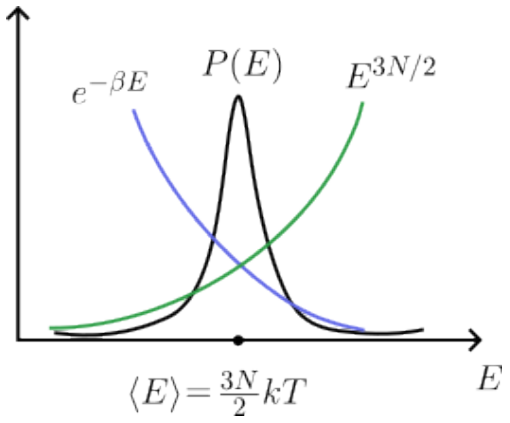
\includegraphics[width=0.35\linewidth]{Immagini/distribuzione P(E).png}
    \caption{grafico della distribuzione di probabilità $P(E)$.}
    \label{fig: distribuzione P(E)}
\end{figure}

\section{Teorema di equipartizione dell'energia}
Si consideri un sistema di $N$ componenti e si supponga che ogni particella sia priva di struttura e sia descrivibile tramite $d$ coppie di variabili coniugate $(q^i,p_i)$ contenute in uno spazio $d$-dimensionale; per cui in totale si hanno $Nd$ coppie ordinate di coordinate $(q^I,p_I)$ con $I = 1,\dots,Nd$. Se si considerano ora le particelle come distinguibili\footnote{In caso contrario tutta la discussione si ripete in modo analogo dopo aver inserito il fattore di indistinguibilità $1/N!$.}, la funzione di partizione è
\begin{equation}
    Z(\beta,V,N) = \int\frac{d^{Nd}q\,d^{Nd}p}{h^{Nd}}e^{-\beta H(q,p)} \equiv \int d\mu\,e^{-\beta H}.
\end{equation}
Ci si concentra ora sull'importante classe di hamiltoniane omogenee di grado secondo nelle $(Nd)$ coordinate di impulso e nelle $Nf_q$ coordinate di posizione non cicliche.
\begin{ex}
    Alcuni esempi di hamiltoniane omogenee di grado secondo sono quella del gas ideale di $N$ componenti in tre dimensioni e quella di $N$ oscillatori armonici unidimensionali disaccoppiati, rispettivamente
    \begin{equation}
        H(q,p) = \sum_{i=1}^N\frac{|\vp_i|^2}{2m},\quad H(q,p) = \sum_{i=1}^N\bigg[\frac{|\vp_{i}|^2}{2m} + \frac{1}{2}m_i w_i^2 (q^i)^2\bigg].
    \end{equation}
\end{ex}
Questa classe di hamiltoniane è importante perchè in tutte le situazioni in cui si devono descrivere piccole fluttuazioni di un sistema intorno ad uno stato di equilibrio, determinato da un minimo del potenziale, si ha un termine cinetico e un termine quadratico nelle coordinate $q$ non cicliche, mentre il termine lineare è assente per la condizione di minimo. Quindi, la classe delle hamiltoniane omogenee di grado due è estremamente rilevante per discutere i sistemi le cui componenti sono libere e/o fluttuano rispetto a posizioni di equilibrio. Sempre per queste hamiltoniane vale la relazione di Eulero
\begin{equation}
\label{eq: relazione di Eulero}
    \bigg(\sum_{I=1}^{Nd}p_I\frac{\p}{\p p_I} + \sum_{J=1}^{Nf_q}q_J\frac{\p}{\p q_J}\bigg)H = 2H,
\end{equation}
il cui valore medio corrisponde a 
\begin{equation}
\label{eq: valore medio relazione di Eulero}
    \vmedio{H(q,p)} \equiv \vmedio{E} = \frac{1}{2}\bigg(\sum_{I=1}^{Nd}\bigvmedio{p_I\frac{\p H}{\p p_I}} + \sum_{J=1}^{Nf_q}\bigvmedio{q^J\frac{\p H}{\p q^J}}\bigg).
\end{equation}
Si consideri il primo termine a secondo membro dell'espressione \eqref{eq: valore medio relazione di Eulero}, in generale si ha
\begin{equation}
    \bigvmedio{p_I\frac{\p H}{\p p_I}} = \frac{1}{Z}\int d\mu\,p_I\frac{\p H}{\p p_I}e^{-\beta H} =  \frac{1}{Z}\int d\mu\, p_I\bigg(-\frac{1}{\beta}\bigg)\frac{\p }{\p p_I}e^{-\beta H},\quad\forall I,
\end{equation}
il quale integrato per parti, osservando che i termini di bordo sono nulli per $p_I\to\pm\infty$ a causa del termine $\exp{(-\beta|\vp_I|^2)/2m}$ in $H$, si ottiene
\begin{equation}
    \bigvmedio{p_I\frac{\p H}{\p p_I}} = \frac{1}{\beta Z}\int d\mu\,\frac{\p p_I}{\p p_I}e^{-\beta H} = \frac{1}{\beta} \equiv kT.
\end{equation}
Quindi, il valore medio rispetto a qualsiasi componente dell'impulso è sempre pari a $kT$. Analogamente, per il secondo termine si ha
\begin{equation}
\label{eq: primo termine valore medio relazione di Eulero}
    \bigvmedio{q^J\frac{\p H}{\p q^J}} = \frac{1}{Z}\int d\mu\,q^J\frac{\p H}{\p q^J}e^{-\beta H} =  \frac{1}{Z}\int d\mu\,q^J\bigg(-\frac{1}{\beta}\bigg)\frac{\p}{\p q^J}e^{-\beta H},\quad\forall J,
\end{equation}
il quale integrato per parti, osservando che i termini di bordo sono nulli in quanto si assume che $H$ contenga il termine di potenziale che cresce con $q^J$ confinando così il sistema, si ottiene nuovamente
\begin{equation}
\label{eq: secondo termine valore medio relazione di Eulero}
    \bigvmedio{q^J\frac{\p H}{\p q^J}} = \frac{1}{\beta Z}\int d\mu\,\frac{\p q^J}{\p q^J}e^{-\beta H} = \frac{1}{\beta} \equiv kT.
\end{equation}
Dunque, sostituendo i risultati ottenuti nella \eqref{eq: primo termine valore medio relazione di Eulero} e \eqref{eq: secondo termine valore medio relazione di Eulero} nella \eqref{eq: valore medio relazione di Eulero}, svolgendo la somma sugli indici $I$ e $J$, si ricava la ``relazione di equipartizione dell'energia'' 
\begin{equation}
\label{eq: relazione di equipartizione dell'energia}
    \vmedio{E} = \frac{1}{2}(Nd + Nf_q)\frac{1}{\beta} = N(d + f_q)\frac{kT}{2}.
\end{equation}
Essenzialmente, la relazione \eqref{eq: relazione di equipartizione dell'energia} afferma che ogni coordinata di tipo $q$ o $p$ che compare nell'hamiltoniana contribuisce all'energia interna con la stessa quantità $kT/2$. 
\begin{obs}
    Dalla \eqref{eq: relazione di equipartizione dell'energia} segue che la capacità termica è indipendente dalla temperatura; infatti
    \begin{equation}
        c_{V,N} = \frac{\p \vmedio{E}}{\p T}\bigg|_{V,N} = N(d + f_q)\frac{k}{2}.
    \end{equation}
    Tuttavia, questo comportamento della capacità termica, inevitabilmente previsto nel contesto classico, è inconsistente con il comportamento reale.
\end{obs}

\section{Teorema del viriale}
Si consideri per semplicità una situazione in cui non sono presenti coordinate cicliche, ossia dove tutte le $\vq^i$ compaiono nell'hamiltoniana, per cui $f_q = d$. Si assuma poi che l'unica dipendenza dagli impulsi sia nel termine cinetico 
\begin{equation}
    K = \sum_{i=1}^{Nd} \frac{|\vp_i|^2}{2m}
\end{equation}
il quale è omogeneo di grado secondo, così che
\begin{equation}
\label{eq: valore medio termine cinetico (teorema viriale)}
    \vmedio{K} = \frac{1}{2} \sum_{i=1}^{Nd} \bigvmedio{p_i \frac{\partial K}{\partial p_i}} = \frac{Nd}{2}kT
\end{equation}
dove nel secondo passaggio si è usata la \eqref{eq: primo termine valore medio relazione di Eulero}. Le equazioni di Hamilton affermano che
\begin{equation}
    \frac{\p H}{\p q_I} = -\dot{p}_I = -F_I, \quad I \equiv (i,a),\,i=1,\cdots,N,\,a = 1,2,3,
\end{equation}
dove $F_I$ è la $a$-esima componente della forza agente sulla $i$-esima particella. Quindi, il ``viriale'' del sistema è definito come
\begin{equation}
    \vps = \nsum_i q^i F_i = \sum_{I=1}^{Nd} q^I F_I,
\end{equation}
il cui valor medio, usando l'equazione di Hamilton per $q^I$, è
\begin{equation}
\label{eq: valore medio viriale (teorema viriale)}
    \vmedio{\vps} = -\nsum_i \bigvmedio{q^i\frac{\partial H}{\partial q^i}} = -NdkT
\end{equation}
avendo usato nell'ultimo passaggio la \eqref{eq: secondo termine valore medio relazione di Eulero}. Confrontando la \eqref{eq: valore medio termine cinetico (teorema viriale)} e la \eqref{eq: valore medio viriale (teorema viriale)} si trova che
\begin{equation}
\label{eq: teorema del viriale}
    \vmedio{\vps} = -2\vmedio{K}.
\end{equation}
L'espressione \eqref{eq: teorema del viriale} è analoga al ``teorema del viriale''\footnote{La prima formulazione del teorema è dovuta a Clausius nel 1870; il nome viriale deriva dal latino ``vis'' significa forza o energia.} in Meccanica classica, il quale afferma che il valor medio temporale del viriale è uguale al doppio del valor medio dell'energia cinetica temporale cambiato di segno, in breve
\begin{equation}    
    \vmedio{\vps}_t = -2\vmedio{K}_t.
\end{equation}

\section{Teorema di Nernst}
L'energia interna termodinamica $E$, corrispondente nell'ensemble canonico a $\vmedio{E}$, è una funzione monotona crescente della temperatura $T$; infatti
\begin{equation}
    c_{V,N} = \frac{\p E}{\p T}\bigg|_{V,N} \ge 0,
\end{equation}
come già era noto a partire dalle condizioni di stabilità termodinamiche e dal legame di $c_{V,N}$ con la varianza $\sigma_E^2$ delle fluttuazioni energetiche \eqref{eq: relazione tra le fluttuazioni di E e cV,N (canonico)}. Quindi, a temperatura $T = 0$, l'energia deve essere la minima possibile e il sistema si deve trovare nello stato fondamentale. Riguardo a quest'ultimo punto si devono distinguere due casi.
\setcounter{caso}{0}
\begin{caso}[stato fondamentale non degenere]
    Se lo stato fondamentale non è degenere, allora ne esiste solamente uno che si indica con $\nu_0$ e la probabilità che il sistema sia in un microstato generico a $T=0$ è semplicemente $P(\nu) = \delta_{\nu,\nu_0}$. In questo caso, l'entropia si annulla dato che il sistema non può cambiare microstato
    \begin{equation}
        \begin{split}
            S = -k\nsum_\nu P(\nu)\log{P(\nu)} = -k\nsum_\nu\delta_{\nu,\nu_0}\log{P(\nu_0)} &= -k\log{P(\nu_0)} \\
            &= -k\log{1} \\
            &= 0.
        \end{split}
    \end{equation}
    Il risultato appena trovato è proprio il contenuto del teorema di Nernst, il quale afferma che l'entropia si annulla allo zero assoluto. Da ciò segue che anche la capacità termica si deve annullare a $T \to 0$, infatti
    \begin{equation}
        c_{V,N} = T\frac{\p S}{\p T} \to 0
    \end{equation}
    dato che $\p S/\p T$ non può divergere per $T \to 0$ dato che $S \to 0$. Il fatto che $c_{V,N} \to 0$ per $T \to 0$ è in netto contrasto con il risultato proveniente dal teorema di equipartizione; tuttavia, l'errore non è qui, ma nell'equipartizione. Infatti, in quel contesto si era ipotizzato che il sistema fosse trattabile classicamente, ma trascurando il fatto che per temperature basse non può essere tralasciata la descrizione quantistica del sistema. Pertanto, l'equipartizione vale solo nel limite classico.
\end{caso}
\begin{caso}[stato fondamentale degenere]
    Se lo stato fondamentale è degenere, allora esistono $m$ stati distinti $\nu_{0,i}$ di energia minima. Avendo tutti la medesima energia, i microstati sono tutti equiprobabili con probabilità $1/m$, per cui
    \begin{equation}
        P(\nu) = 
        \begin{cases}
            1/m,\quad \forall i =1,\dots,m \\
            0,\quad \nu \neq \nu_{0,i}
        \end{cases}.
    \end{equation}
    In questo caso, l'entropia non si annulla allo zero assoluto, ma compare un'entropia ``residua''
    \begin{equation}
        S = -k\nsum_{i = 1}^mP(\nu_{0,i})\log{P(\nu_{0,i})} = -\frac{k}{m}\nsum_{i = 1}^m\log{\frac{1}{m}} = k\log{m}.
    \end{equation}
    Normalmente, il numero di microstati degeneri $m$ non è proporzionale ad $N$ e l'entropia residua è presente ma è molto piccola nel limite termodinamico.
\end{caso}

\section{Solido di Einstein nell'ensemble canonico}
Come già visto nell'ensemble microcanonico, il solido di Einstein è un modello che consiste in $3N$ oscillatori armonici quantistici di frequenza $\omega$ disaccoppiati. Gli $N$ componenti sono non interagenti e indistinguibili, per cui la funzione di partizione del sistema si fattorizza\footnote{Non c'è bisogno di introdurre il fattore di Gibbs dato che gli elementi sono indistinguibili, come prescrive la Meccanica quantistica.} in $Z = [Z_{(1)}]^{3N}$, dove $Z_{(1)}$ è la funzione di partizione del singolo oscillatore armonico quantistico di frequenza $\omega$. Si indica con $\{\ket{n}\}$ a base degli autostati dell'energia per l'oscillatore armonico e si rappresenta la matrice densità in tale base
\begin{equation}
    \rho_{mn} = \frac{e^{-\beta E_n}} {Z_{(1)}}\delta_{mn},\quad Z_{(1)} = \Tr{\hatrho} = \nsum_n e^{-\beta E_n}.
\end{equation}
Dato che gli autostati dell'energia non sono degeneri, l'energia associata vale
\begin{equation}
    E_n = \bigg(n + \frac{1}{2}\bigg)\hbar\omega.
\end{equation}
Quindi, si ha che la funzione di partizione parziale, usando la nozione di serie geometrica, è
\begin{equation}
\label{eq: funzione di partizione singola particella solido di Einstein (canonico)}
    \begin{split}
        Z_{(1)} = \nsum_n e^{-\beta(n + 1/2)\hbar\omega} &= e^{-\beta\hbar\omega/2}\nsum_n(e^{-\beta\hbar\omega})^n \\
        &= \frac{e^{-\beta\hbar\omega}}{1 - e^{-\beta\hbar\omega}} \\
        &= \bigg(2\sinh{\frac{\beta\hbar\omega}{2}}\bigg)^{-1},
    \end{split}
\end{equation}
da cui segue immediatamente che
\begin{equation}
    Z = \bigg(2\sinh{\frac{\beta\hbar\omega}{2}}\bigg)^{-3N}.
\end{equation}
Ora, ottenuta la funzione di partizione del sistema, è possibile ricavare tutte le grandezze termodinamiche. Prima di tutto, l'energia libera è data da
\begin{equation}
    F = -\frac{\log{Z}}{\beta} = \frac{3N}{\beta}\log{\bigg(2\sinh{\frac{\beta\hbar\omega}{2}}\bigg)};
\end{equation}
invece, l'energia termodinamica è
\begin{equation}
    E \equiv \vmedio{E} = -\frac{\p\log{Z}}{\p\beta} = \frac{3N\hbar\omega}{2}\coth{\frac{\beta\hbar\omega}{2}} = 3N\hbar\omega\bigg(\frac{1}{e^{\beta\hbar\omega} - 1} + \frac{1}{2}\bigg),
\end{equation}
in accordo con quanto trovato nell'ensemble microcanonico con la \eqref{eq: energia solido di Einstein (microcanonico)}. Chiaramente, nel regime di alta temperatura si ritrova il risultato classico $\vmedio{E} = 3NkT$ per $kT \gg \hbar\omega$, ricavabile dal teorema di equipartizione per $3N$ oscillatori con $d = 1$ e $f_q = 1$.

\subsection{Rotazione di Wick}
Esiste una profonda relazione tra la trattazione statistica di un sistema quantistico e la ``rotazione di Wick'', una particolare trasformazione agente sulla coordinata temporale. Si consideri quindi un sistema quantistico con un solo grado di libertà $q$, che si può pensare come singola componente di un sistema non interagente. 
\begin{obs}
    Per sistemi interagenti si dovrebbero considerare innumerevoli gradi di libertà; formalmente la generalizzazione non è un problema.
\end{obs}
Siano $\ket{q}$ gli autostati dell'operatore posizione e $\ket{q(t)}$ i corrispondenti stati nella descrizione di Schr\"odinger che evolvono nel tempo tramite
\begin{equation}
    \ket{q(t)} = e^{i\hatH t/\hbar}\ket{q}.
\end{equation}
Si introduce ora il ``nucleo'', o ``kernel'', $K(q_f,q_i;t_f,t_i)$ come
\begin{equation}
\label{eq: definizione kernel}
    K(q_f,q_i;t_f,t_i) = \mybraket{q_f(t_f)}{q_i(t_i)},
\end{equation}
il quale descrive la probabilità che il sistema si trovi nella posizione $q_f$ al tempo $t_f$ a partire dalla posizione $q_i$ al tempo $t_i$. Si supponga ora di effettuare una rotazione di Wick rimpiazzando il tempo $t$ con il ``tempo euclideo'' $\tau \in \R$ secondo la trasformazione $t \to -i\tau$. In questo modo, il kernel \eqref{eq: definizione kernel} diventa il kernel euclideo
\begin{equation}
    K_E(q_f,q_i;\Delta\tau = \tau_f - \tau_i) = \mybrakett{q_f}{e^{-\Delta\tau\hatH/\hbar}}{q_i},
\end{equation}
dove il fattore di evoluzione temporale diventa una fattore di Boltzmann ponendo
\begin{equation}
    \frac{\Delta\tau}{\hbar} = \frac{1}{kT} \equiv \beta,
\end{equation}
arrivando così all'espressione
\begin{equation}
\label{eq: kernel euclideo}
     K_E(q_f,q_i;\Delta\tau = \hbar\beta) = \mybrakett{q_f}{e^{-\beta\hatH}}{q_i}.
\end{equation}
Quindi, il kernel è essenzialmente la matrice densità nella base della posizione con il tempo $\Delta\tau$. Se si definisce la funzione di partizione come la traccia del kernel \eqref{eq: kernel euclideo}, ossia ponendo $q_f = q_i \equiv q$, allora
\begin{equation}
\label{eq: funzione di partizione come traccia del kernel euclideo (canonico)}
    Z_E = \int dq\,K_E(q,q;\Delta\tau) = \int dq\,\mybrakett{q}{e^{-\beta\hatH}}{q} = \Tr{e^{-\beta\hatH}}
\end{equation}
ed è evidente come questa corrisponda alla funzione di partizione canonica, con la traccia presa nella base $\{\ket{q}\}$ degli autostati della posizione. Dalle equazioni \eqref{eq: kernel euclideo} e \eqref{eq: funzione di partizione come traccia del kernel euclideo (canonico)} segue che la matrice densità in tale base è
\begin{equation}
\label{eq: matrice densità in termini del kernel (canonico)}
    \rho_{q_f,q_i} = \frac{1}{Z}K_E(q_f,q_i;\Delta\tau).
\end{equation}
Il kernel può essere espresso in vari modi, uno di questi è tramite l'integrale funzionale
\begin{equation}
\label{eq: kernel come integrale funzionale}
    K(q_f,q_i;t_f,t_i) = \int_{q(t_i)}^{q(t_f)} Dq\,e^{iS[q(t)]/\hbar}.
\end{equation}
L'idea di usare un integrale di cammino si fonda sulla possibilità di in Meccanica quantistica di passare dalla posizione iniziale a quella finale facendo un integrale sulle traiettorie, opportunamente pesate da un esponenziale dipendente dal funzionale di azione $S[q(t)]$. Tra tutte le possibili traiettorie, quella corrispondente alla traiettoria classica è quella con il peso maggiore, tutte le altre avranno un peso minore di questa. Rispetto ad una rotazione di Wick, si può definire l'azione euclidea $S_E[q(t)]$ come
\begin{equation}
    iS[q(t)] \to -S_E[q(\tau)],\quad t \to -i\tau.
\end{equation}
In questo modo, la funzione di partizione \eqref{eq: funzione di partizione come traccia del kernel euclideo (canonico)} diventa anch'essa euclidea
\begin{equation}
\label{eq: funzione di partizione come integrale funzionale euclideo (canonico)}
    Z_E = \int_{PBC}Dq\,e^{-S_E[q(\tau)]/\hbar},
\end{equation}
dove le funzioni $q(\tau)$ obbediscono alle ``periodic boundary conditions'' (PBC) definite da
\begin{equation}
\label{eq: PBC}
    q(\tau_i) = q(\tau_f) = q(\tau_i + \Delta\tau) = q(\tau_i + \hbar\beta).
\end{equation}
Si nota che proprio in queste condizioni al bordo entra in gioco la temperatura del sistema. La funzione di partizione dell'integrale canonico a temperatura $T$ può quindi essere calcolata tramite l'integrale funzionale euclideo \eqref{eq: funzione di partizione come integrale funzionale euclideo (canonico)} imponendo le condizioni al bordo periodiche \eqref{eq: PBC}. Geometricamente, la funzione di partizione così definita corrisponde alla ``compattificazione'' del tempo euclideo su un cerchio di lunghezza $\hbar\beta$, come rappresentato in figura \ref{fig: compattificazione tempo euclideo}.
\begin{figure}[h]
    \centering
    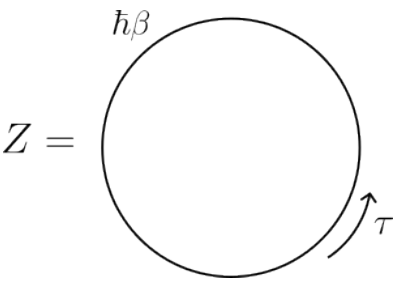
\includegraphics[width=0.35\linewidth]{Immagini/compattificazione tempo euclideo.png}
    \caption{compattificazione del tempo euclideo su un cerchio $S_1$.}
    \label{fig: compattificazione tempo euclideo}
\end{figure}

Analogamente alla \eqref{eq: funzione di partizione come integrale funzionale euclideo (canonico)}, anche il kernel euclideo può essere espresso in funzione di $S_E$ tramite
\begin{equation}
\label{eq: kernel euclideo come integrale funzionale}
    K_E(q_f,q_i;\tau_f,\tau_i) = \int_{q(\tau_i)}^{q(\tau_f)} Dq\,e^{-S_E[q(\tau)]/\hbar}.
\end{equation}
Tramite la \eqref{eq: matrice densità in termini del kernel (canonico)}, la conoscenza del kernel euclideo e della funzione di partizione euclidea fornisce la matrice densità nella base degli autostati della posizione. Tuttavia, la matrice può anche essere calcolata a partire dalla base dell'energia; infatti, se $\{\ket{n}\}$ sono gli stati stazionari, sfruttando la relazione di completezza nella \eqref{eq: kernel euclideo}, si ha
\begin{equation}
\label{eq: kernel in termini delle funzioni d'onda stati stazionari (canonico)}
    \begin{split}
        K_E(q_f,q_i;\Delta\tau) &= \nsum_n\mybraket{q_f}{n}\mybrakett{n}{e^{-\beta\hatH}}{q_i} \\
        &= \nsum_n\mybraket{q_f}{n}\mybraket{n}{q_i}e^{-\beta E_n} \\
        &= \nsum_n u^*_n(q_f)u_n(q_i)e^{-\beta E_n},
    \end{split}
\end{equation}
dove le $u_n(q)$ sono le funzioni d'onda degli stati stazionari.
\begin{ex}
    Per un oscillatore armonico quantistico di frequenza $\omega$, l'azione è
    \begin{equation}
        iS[q(t)] = i\int_{t_i}^{t_f} dt\,\bigg(\frac{m}{2}\dot{q}^2 - \frac{1}{2}m\omega^2q^2\bigg),
    \end{equation}
    la quale sotto rotazione di Wick diventa l'azione euclidea
    \begin{equation}
        S_E[q(\tau)] = \int_{\tau_i}^{\tau_f}d\tau\,\bigg[\frac{m}{2}\bigg(\frac{dq}{d\tau}\bigg)^2 + \frac{1}{2}m\omega^2q^2\bigg].
    \end{equation}
    Di conseguenza, il kernel euclideo è
    \begin{equation}
        K_E(q_f,q_i;\Delta\tau) = \int_{q(\tau_i)}^{q(\tau_f)}Dq(\tau)\,\exp{\bigg\{-\int_{\tau_i}^{\tau_f}d\tau\,\bigg[\frac{m}{2}\bigg(\frac{dq}{d\tau}\bigg)^2 + \frac{1}{2}m\omega^2q^2\bigg]\bigg\}}.
    \end{equation}
    Questo può essere calcolato esplicitamente dividendo $q(\tau)$ in una traiettoria classica $q(\tau)_c$ che soddisfa le equazioni del moto e in una fluttuazione quantistica $x(\tau)$, per cui $q(\tau) := q(\tau)_c + x(\tau)$. Il passo successivo è il calcolo dell'integrale funzionale sulle fluttuazioni, omettendo questo passaggio per semplicità, il risultato finale è
    \begin{equation}
        \begin{split}
            K_E(q_f,q_i;\Delta\tau) &= \sqrt{\frac{m\omega}{2\pi\hbar\sinh{\beta\hbar\omega}}} \\
            &\times\exp{\bigg\{-\frac{m\omega}{2\hbar\sinh{\beta\hbar\omega}}[(q_i^2 + q_f^2)\cosh{(\beta\hbar\omega) - 2q_iq_f}]\bigg\}}.
        \end{split}
    \end{equation}
    A questo punto, la funzione di partizione è direttamente ricavabile dalla \eqref{eq: funzione di partizione come integrale funzionale euclideo (canonico)}; l'espressione da risolvere è un integrale gaussiano, il cui risultato è
    \begin{equation}
        Z = \bigg(2\sinh{\frac{\beta\hbar\omega}{2}}\bigg)^{-1},
    \end{equation}
    in perfetto accordo con quanto trovato nella \eqref{eq: funzione di partizione singola particella solido di Einstein (canonico)}. La relazione \eqref{eq: matrice densità in termini del kernel (canonico)} permette di determinare la matrice densità nella base delle posizioni; in particolare, i termini diagonali di $\rho_{qq}$ che rappresentano la probabilità che l'oscillatore ``termalizzato'' si trovi nella posizione $q$ sono dati da
    \begin{equation}
        \begin{split}
            \rho_{qq} &= 2\sinh{\frac{\beta\hbar\omega}{2}}\sqrt{\frac{m\omega}{2\pi\hbar\sinh{\beta\hbar\omega}}}\exp{\bigg\{-\frac{2m\omega\sinh{(\beta\hbar\omega/2)}}{\hbar\sinh{\beta\hbar\omega}}q^2\bigg\}} \\
            &= \sqrt{\frac{m\omega}{\pi\hbar}\tanh{\frac{\beta\hbar\omega}{2}}}\exp{\bigg\{-\frac{m\omega}{\hbar}\tanh{\bigg(\frac{\beta\hbar\omega}{2}\bigg)}q^2\bigg\}},
        \end{split}
    \end{equation}
    dove si è usata la relazione trigonometrica
    \begin{equation}
        \sinh{\beta\hbar\omega} = 2\sin{\bigg(\frac{\beta\hbar\omega}{2}\bigg)}\cos{\bigg(\frac{\beta\hbar\omega}{2}\bigg)}.
    \end{equation}
\end{ex}

\subsection{Condizioni al bordo periodiche}
L'obiettivo adesso è dimostrare che nel limite termodinamico la forma delle condizioni al contorno è irrilevante e, di conseguenza, è possibile scegliere le condizioni al contorno più convenienti a seconda del sistema in esame. Per semplicità, si considera un gas di particelle quantistiche non interagenti, la cui funzione di partizione si fattorizza secondo \eqref{eq: funzione di partizione sistemi non interagenti (canonico)} in termini di quella associata alla singola particella $Z_{(1)}$. Ancora per motivi di semplicità, si suppone che il gas sia confinato in un cubo di lato $L$; comunque, in ogni caso è possibile dimostrare che anche la forma del volume contente il sistema è irrilevante. Essendo la particella libera, il problema tridimensionale si decompone in tre copie del problema di una particella confinata in una buca infinita di potenziale unidimensionale. Le autofunzioni dell'hamiltoniana $\hatH = -(-\hbar^2/2m)\nabla^2$ sono
\begin{equation}
\label{eq: funzione d'onda stati stazionari buca di potenziale (canonico)}
    u_n(x) = \sqrt{\frac{2}{L}}\sin{k_n x},\quad k_n \equiv \frac{\pi n}{L},
\end{equation}
le quali soddisfano le condizioni di annullamento $u_n(0) = u_n(L) = 0$ e sono tali che 
\begin{equation}
\label{eq: energie stati stazionari buca di potenziale (canonico)}
    \hatH u_n = E_nu_n,\quad E_n = \frac{(\hbar\pi n)^2}{2mL} \equiv n^2 E_1,
\end{equation}
oltre ad essere normalizzate tramite
\begin{equation}
    \int_0^L dx\,|u_n(x)|^2 = 1.
\end{equation}
I livelli di energia non sono degeneri, per cui la funzione di partizione vale
\begin{equation}
\label{eq: funzione di partizione particella buca di potenziale (canonico)}
    Z_x = \nsum_n e^{-\beta E_n} = \nsum_n e^{-\beta n^2E_1}.
\end{equation}
Si nota adesso che il termine $\beta E_1$ può essere espresso in termini della lunghezza d'onda termica $\lambda_T$ introdotta nella \eqref{eq: funzione di partizione singola particella (canonico)}, infatti
\begin{equation}
    \beta E_1 = \frac{\beta\hbar^2\pi^2}{2mL^2} = \frac{\pi}{4}\frac{\beta h^2}{2\pi m}\frac{1}{L^2} = \frac{\pi}{4}\bigg(\frac{\lambda_T}{L}\bigg)^2.    
\end{equation}
L'espressione \eqref{eq: funzione di partizione particella buca di potenziale (canonico)} è esatta, tuttavia si può considerare il suo sviluppo in due casi diversi.
\setcounter{caso}{0}
\begin{caso}[bassa temperatura]
    Nel limite di bassa temperatura, l'energia termica è molto minore dell'energia dello stato fondamentale del sistema, per cui
    \begin{equation}
        kT \ll E_1 \quad\Longleftrightarrow\quad \lambda_T \gg L.
    \end{equation}
    In questo regime la soppressione esponenziale nella \eqref{eq: funzione di partizione particella buca di potenziale (canonico)} è estremamente efficace e quindi
    \begin{equation}
    \label{eq: sviluppo bassa T funzione di partizione particella buca di potenziale (canonico)}
        Z_x = e^{-\beta E_1} + e^{-4\beta E_1} + \cdots \simeq e^{-(\pi/4)(\lambda_T/L)^2},
    \end{equation}
    per cui la funzione di partizione riceve quasi esclusivamente il contributo dello stato fondamentale. Questo risultato non è di particolare interesse, se non per il fatto che classicamente non è prevista una tale situazione.
\end{caso}
\begin{caso}[alta temperatura]
    Nel limite di alta temperatura, ci si aspetta di ritrovare il risultato derivato dalla trattazione classica; in questo caso
    \begin{equation}
        kT \gg E_1 \quad\Longleftrightarrow\quad \lambda_T \ll L.
    \end{equation}
    Questa volta, la soppressione esponenziale nella \eqref{eq: funzione di partizione particella buca di potenziale (canonico)} non è così efficace in quanto adesso tutti gli elementi della serie contribuiscono a $Z_x$; pertanto, è necessario risommare la serie tramite la ``risommazione di Poisson'', di seguito esposta.
    \begin{teo}[Risommazione di Poisson]
        Data una funzione $f(x)$ e sia $\tilde{f}(p)$ la sua antitrasformata di Fourier data da
        \begin{equation}
            \tilde{f}(p) = \int dx\,e^{-ipx}f(x),
        \end{equation}
        allora vale la formula
        \begin{equation}
        \label{eq: risommazione di Poisson}
            \sum_{n\in\Z}f(n) = \sum_{r\in\Z}\tilde{f}(2\pi r).
        \end{equation}
    \end{teo}
    Quindi, si riscrive la funzione di partizione \eqref{eq: funzione di partizione particella buca di potenziale (canonico)} come\footnote{Si vuole la sommatoria su tutti gli interi, ma in $Z$ si ha solo quella sugli interi positivi. Però, essendo pari, si può riscrivere $Z$ come la somma $(1/2)\nsum_n$. Tuttavia, facendo la somma su tutti gli $n$ si considera anche il caso non interessante $n = 0$, per cui lo si sottrae considerando che $e^0 = 1$.}
    \begin{equation}
        Z_x = \frac{1}{2}\bigg(\sum_{n\in\Z}e^{-(\pi/4)(\lambda_T/L)^2n^2} - 1\bigg) \equiv \frac{1}{2}\bigg(\sum_{n\in\Z}f(n) - 1\bigg),
    \end{equation}
    applicando la formula di Poisson \eqref{eq: risommazione di Poisson} con 
    \begin{equation}
        \tilde{f}(r) = \int dn\,e^{-irn}e^{-(\pi/4)(\lambda_T/L)^2n^2} = \frac{2L}{\lambda_T}e^{-r^2L/\lambda_T\pi},
    \end{equation}
    ottenendo così 
    \begin{equation}
        Z_x = \frac{1}{2}\bigg(\frac{2L}{\lambda_T}\sum_{r\in\Z}e^{-4\pi r^2(L/\lambda_T)^2} - 1\bigg).
    \end{equation}
    Quindi, nel limite di alta temperatura si ha che $L/\lambda_T \gg 1$ e quindi ora la soppressione esponenziale è efficace
    \begin{equation}
    \label{eq: sviluppo alta T funzione di partizione particella buca di potenziale  (canonico)}
        Z_x \simeq \frac{1}{2}\bigg[\frac{2L}{\lambda_T}(1 + \cdots) - 1\bigg] \simeq \frac{L}{\lambda_T}\bigg(1 - \frac{\lambda_T}{2L} + \cdots \bigg) \simeq \frac{L}{\lambda_T}.
    \end{equation}
    Questo risultato corrisponde al caso classico, infatti dato che $Z_x  = Z_y = Z_z$, in tre dimensioni si ottiene proprio \eqref{eq: funzione di partizione singola particella (canonico)}.
\end{caso}
\begin{obs}
    Esiste un modo più semplice per ottenere lo stesso risultato per il termine dominante\footnote{La risommazione di Poisson permette di ottenere anche tutti i termini sottodominanti, ma in questo caso non sono di particolare interesse.}. Quest'ultimo si ottiene se si sostituisce la sommatoria su $n$ nella \eqref{eq: funzione di partizione particella buca di potenziale (canonico)} con un integrale, cioè facendone il limite al continuo. Infatti, nel limite di alta temperatura i livelli quantistici sono quasi continui. Per fare, si usa la formula di Eulero-MacLaurin\footnote{La formula di Eulero-MacLaurin è 
    \begin{equation}
        \sum_{n = p+1}^qf(n) = \int_p^q dn\,f(n) + \sum_{k=1}^r\frac{B_k}{k!}[f^{(k-1)}(q) - f^{(k-q)}(p)] + R_r,
    \end{equation}
    dove i $B_k$ sono i ``numeri di Bernoulli''.}, così si ha
    \begin{equation}
        \nsum_n \longrightarrow \int dn = \frac{L}{\pi} \int dk,
    \end{equation}
    dove si è introdotto il numero d'onda continuo $k$ per rimpiazzare i valori discreti $k_n$. Quindi, dalla \eqref{eq: funzione di partizione particella buca di potenziale (canonico)} si ottiene un integrale gaussiano e il medesimo risultato
    \begin{equation}
        \begin{split}
            Z_x \simeq \frac{1}{2} \bigg( \frac{L}{\pi} \int_\R dk\, e^{-\lambda_T^2k^2/4\pi^2} - 1 \bigg) &= \frac{1}{2} \bigg( \frac{L}{\pi} \sqrt{\frac{4\pi^2}{\lambda_T^2}} - 1 \bigg)  \\
            &= \frac{1}{2} \bigg( \frac{2L}{\lambda_T} - 1 \bigg) \\
            &\simeq \frac{L}{\lambda_T}.
        \end{split}
    \end{equation}
\end{obs}
Ora si supponga di imporre delle condizioni al bordo periodiche generiche, anche se non sarebbero adatte al problema della particella confinata in una buca infinita di potenziale $u(x) = u(x + L)$; con tali condizioni, gli stati stazionari hanno come funzione d'onda
\begin{equation}
    \tilde{u}_n(x) = \frac{1}{\sqrt{L}}e^{i\tilde{k_n}x},\quad \tilde{k}_n = \frac{2\pi n}{L}
\end{equation}
ed energie
\begin{equation}
    \tilde{E}_n = \frac{\hbar^2\tilde{k}_n^2}{2m} = n^2\tilde{E}_1.
\end{equation}
Dal confronto con la \eqref{eq: energie stati stazionari buca di potenziale (canonico)} segue immediatamente che
\begin{equation}
    \tilde{E}_n = 4E_n.
\end{equation}
La funzione di partizione è
\begin{equation}
\label{eq: funzione di partizione particella buca di potenziale tilde (canonico)}
    \tilde{Z}_x  =\sum_{n\in\Z}e^{-\beta \tilde{E}_n} = \sum_{n\in\Z}e^{-\beta \tilde{E}_1n^2},\quad \beta\tilde{E}_1 = -\pi\bigg(\frac{\lambda_T}{L}\bigg)^2.
\end{equation}
La sommatoria che appare nell'espressione esatta \eqref{eq: funzione di partizione particella buca di potenziale tilde (canonico)} corrisponde ad una delle ``costanti $\theta$ di Jacobi'' molto importanti in Matematica; in particolare, corrisponde alla $\theta_3$ definita come
\begin{equation}
\label{eq: definizione funzione theta3 di Jacobi}
    \theta_3(v|\tau) = \sum_{n\in\Z}e^{i\pi\tau n^2 + 2\pi ivn} \equiv \theta_3(\tau)\sum_{n\in\Z}e^{2\pi ivn}.
\end{equation}
Quindi, si può scrivere la \eqref{eq: funzione di partizione particella buca di potenziale tilde (canonico)} come 
\begin{equation}
    \tilde{Z}_x = \theta_3\bigg(\frac{i\beta\tilde{E}_1}{\pi}\bigg) = \theta_3\bigg[i\bigg(\frac{\lambda_T}{L}\bigg)^2\bigg],
\end{equation}
su cui è possibile applicare la risommazione di Poisson. Sulle costanti $\theta$ di Jacobi tale risommazione equivale alla proprietà di ``dualità'', che consiste in
\begin{equation}
    \theta_3(\tau) = (-i\tau')^{1/2}\theta_3(\tau'),\quad \tau \to \tau' = -\tau^{-1}.
\end{equation}
Essenzialmente, la $\theta_3$ valutata su un certo argomento è collegata in modo semplice alla $\theta_3$ valutata nell'inverso di tale argomento; in questo caso
\begin{equation}
    \tau = i\bigg(\frac{\lambda_T}{L}\bigg)^2 \to \tau ' = -\bigg(i\frac{\lambda_T}{L}\bigg)^{-2}.
\end{equation}
Detto ciò, come prima si devono distinguere i due limiti un funzione della temperatura.
\setcounter{caso}{0}
\begin{caso}[bassa temperatura]
    Nel limite di bassa temperatura, l'espansione di $\tilde{Z}_x$ è molto diversa da quella di $Z_x$ riportata in \eqref{eq: sviluppo bassa T funzione di partizione particella buca di potenziale (canonico)}, infatti ora
    \begin{equation}
        \tilde{Z}_x = 1 + 2e^{-\beta\tilde{E}_1} + \cdots = 1 + 2e^{-\pi\lambda_T^2/L^2} + \cdots,
    \end{equation}
    dove il termine esponenziale non è dominante. Quindi, in questo limite la particella si trova quasi sicuramente nello stato fondamentale, e questi con le due diverse condizioni al contorno sono diversi.
\end{caso}
\begin{caso}[alta temperatura]
    Nel limite di alta temperatura si può effettuare la risommazione di Poisson ottenendo
    \begin{equation}
        \begin{split}
            \tilde{Z}_x = \sum_{n\in\Z} e^{-\pi(\lambda_T/L)^2n^2} &= \frac{L}{\lambda_T}\sum_{r\in\Z}e^{-\pi(L/\lambda_T)^2r^2} \\
            &= \frac{L}{\lambda_T}\bigg[1 + 2e^{-\pi(L/\lambda_T)^2} + \cdots\bigg] \\
            &\simeq Z_x.
        \end{split}
    \end{equation}
    Dunque, in questo limite le funzioni di partizione calcolate con diverse condizioni al contorno coincidono: per un sistema con molte componenti di questo tipo la termodinamica da esse derivata è la medesima. In realtà non è proprio così, in quanto potrebbero esistere alcune osservabili localizzate vicino al bordo più sensibili al fatto di aver cambiato le condizioni al contorno. Per questo si dice che le condizioni al contorno sono ``quasi irrilevanti''.
\end{caso}

\subsubsection{Generalizzazione unidimensionale}
Il fatto che le condizioni siano quasi irrilevanti può essere generalizzato. Per modellizzare il comportamento termodinamico descritto dall'energia libera $F(T,V,N,\dots)$ si può fissare il volume $V$ del sistema confinandolo in una regione qualsiasi forma sia più conveniente, assegnando condizioni al contorno altrettanto vantaggiose per l'analisi. Tuttavia, questo non significa che tutte le osservabili siano indipendenti dalle condizioni al contorno; infatti, una generica osservabile $O$ ha un valore medio statistico dato da
\begin{equation}
    \vmedio{\hatO} = \Tr{\hatO\hatrho},\quad\hatrho = \frac{e^{-\beta\hatH}}{Z}.
\end{equation}
L'operatore densità, ad esempio rappresentato tramite la matrice associata nella base degli autostati della posizione $\rho(x',x) = \mybrakett{x'}{\hatrho}{x}$, in generale dipende dalle condizioni al contorno, influenzando di conseguenza il calcolo delle osservabili localizzate nei pressi del bordo del sistema. 

Si riconsideri il caso della particella quantistica confinata in una buca infinita di potenziale, dalla \eqref{eq: kernel in termini delle funzioni d'onda stati stazionari (canonico)} si ha
\begin{equation}
    \rho(x',x) = \mybrakett{x'}{\hatrho}{x} = \frac{1}{Z_x}\nsum_nu_n^*(x')u_n(x)e^{-\beta E_n}
\end{equation}
che, con la \eqref{eq: funzione d'onda stati stazionari buca di potenziale (canonico)} e la \eqref{eq: energie stati stazionari buca di potenziale (canonico)}, diventa
\begin{equation}
\label{eq: matrice densità buca di potenziale (canonico)}
    \rho(x',x) = \frac{2}{Z_xL}\nsum_n\sin{(kx')}\sin{(kx)}e^{-\lambda_T^2k^2/4\pi},\quad k = \frac{n\pi}{L}.
\end{equation}
Nel limite di alta temperatura, si può passare al continuo tramite la formula di Eulero-MacLaurin, ottenendo
\begin{equation}
    \rho(x',x) = \frac{2}{Z_x\cancel{L}}\frac{\cancel{L}}{\pi}\int_0^\infty dk\,\sin{(kx')}\sin{(kx)}e^{-\lambda_T^2k^2/4\pi}.
\end{equation}
Il risultato finale dell'integrale, di cui si omettono i passaggi di risoluzione per semplicità, è
\begin{equation}
    \rho(x',x) = \frac{1}{Z_x\lambda_T}\bigg[e^{-\pi(x' - x)^2/\lambda_T^2} - e^{-\pi(x' + x)^2/\lambda_T^2} \bigg].
\end{equation}
In particolare, si osserva che
\begin{equation}
    \rho(x',x) = 0\quad\Longleftrightarrow\quad
    \begin{cases}
        x' = 0 \\
        x = 0
    \end{cases}\quad
    \vee\quad
    \begin{cases}
        x' \simeq L \to \infty \\
        x \simeq L \to \infty
    \end{cases}.
\end{equation}
Questo è consistente con il fatto che si sta descrivendo il sistema con condizioni di annullamento ai bordi, per le quali si deve avere ampiezza di transizione nulla quando ci si trova sul bordo. Invece, i termini diagonali di $\rho(x',x)$ rappresentano la probabilità di trovare la particella termalizzata nella posizione $x = x'$
\begin{equation}
    \rho(x,x) = \frac{1}{Z_x\lambda_T}\bigg(1 - e^{-4\pi x^2/\lambda_T^2}\bigg).
\end{equation}
Dall'espressione di $\rho(x,x)$ si deduce che la distribuzione della probabilità per una particella in scatola è sostanzialmente piatta, eccetto in una regione di dimensione $\lambda_T$ vicino al bordo. Tenendo conto che nel limite di alta temperatura $Z_x\lambda_T \simeq L$ e limitandosi a valori di $x$ ed $x'$ non vicini al bordo, si ha che
\begin{equation}
\label{eq: matrice densità buca di potenziale alta T (canonico)}
    \rho(x',x) \simeq \frac{1}{L}e^{-\pi(x' - x)^2/\lambda_T^2}.
\end{equation}

Si passa adesso determinare la matrice densità che si ottiene imponendo delle condizioni al contorno periodiche. In tal caso, l'analgo della \eqref{eq: matrice densità buca di potenziale (canonico)} usando le \eqref{eq: funzione d'onda stati stazionari buca di potenziale (canonico)} e \eqref{eq: energie stati stazionari buca di potenziale (canonico)}, è
\begin{equation}
    \tilde{\rho}(x',x) = \frac{1}{\tilde{Z}_x}\nsum_n\tilde{u}_n^*(x')\tilde{u}_n(x)e^{-\beta\tilde{E}_n} = \frac{1}{\tilde{Z}_xL}\nsum_ne^{-ik_n(x'-x)}e^{-\pi\lambda_T^2/L^2n^2}.
\end{equation}
Sostituendo la somma discreta con un integrale tramite la formula di Eulero-MacLaurin, nel limite di alta temperatura, si ha
\begin{equation}
\label{eq: matrice densità buca di potenziale alta T tilde (canonico)}
    \begin{split}
        \tilde{\rho}(x',x) &= \frac{1}{\tilde{Z}_x\cancel{L}}\frac{\cancel{L}}{2\pi}\int_\R dk\, e^{-ik(x'-x) - \lambda_T^2k^2/4\pi} \\
        &= \frac{1}{\cancel{2\pi}\tilde{Z}_x}\frac{\cancel{2\pi}}{\lambda_T}e^{-\pi(x'-x)^2/\lambda_T} \\
        &\simeq \frac{1}{L}e^{-\pi(x'-x)^2/\lambda_T^2},
    \end{split}
\end{equation}
la quale coincide esattamente con la $\rho(x',x)$ trovata con le condizioni di annullamento al bordo nella \eqref{eq: matrice densità buca di potenziale alta T (canonico)}, per tutte le $x'$ ed $x$ che non si trovano nei pressi del bordo. Dunque, si nota che in precedenza la matrice densità aveva dei termini che non erano trascurabili nei pressi del bordo, adesso invece questo non accade essendo la $\rho$ nella \eqref{eq: matrice densità buca di potenziale alta T tilde (canonico)} periodica e quindi tutti i punti sono uguali. Pertanto, le differenze determinate dalle condizioni al contorno sono minime e sono solo locali. Tendenzialmente d'ora in poi ci si concentra sulle proprietà termodinamiche ``di bulk'', ossia  non legate ad osservabili localizzate presso il bordo, e si scelgono usualmente condizioni di periodicità
che semplificano i calcoli.

\subsubsection{Generalizzazione tridimensionale}
Si generalizza ora al caso tridimensionale. Sempre nel caso in cui la particella sia confinata in un cubo di di volume $V = L^3$, le autofunzioni di energia sono il prodotto di quelle trovate per ciascuna direzione $x, y, z$. Nel caso periodico si ha
\begin{equation}
    \tilde{u}_{\vn}(\vx) = \frac{1}{\sqrt{V}} \tilde{u}_{n_x}(x)\tilde{u}_{n_y}(y)\tilde{u}_{n_z}(z) = \frac{1}{\sqrt{V}} e^{i\vk(\vn)\cdot \vx},\quad k(\vn) = \frac{2\pi}{L}\vn
\end{equation}
dove $\vn = (n_x, n_y, n_z) \in \Z^3$. L'energia è semplicemente la somma di quelle relative alle tre direzioni
\begin{equation}
    \begin{split}
        E_{\vn} = \frac{\hbar^2}{2m}(k_x^2 + k_y^2 + k_z^2) &= \frac{\hbar^2}{2m}\left(\frac{2\pi}{L}\right)^2 (n_x^2 + n_y^2 + n_z^2) \\
        &= \frac{\hbar^2}{2m}|\vk|^2 \\
        &= \frac{h^2}{2m}\left(\frac{2\pi}{L}\right)^2 |\vn|^2.
    \end{split}
\end{equation}
Quindi, la funzione di partizione si fattorizza come
\begin{equation}
    \label{eq: funzione di partizione buca di potenziale tilde 3D (canonico)}
    \begin{split}
        Z = \tilde{Z}_x \tilde{Z}_y \tilde{Z}_z &= \sum_{n_x,n_y,n_z\in\mathbb{Z}} \exp{\bigg[-\beta \frac{\hbar^2}{2m}\left(\frac{2\pi}{L}\right)^2 (n_x^2+n_y^2+n_z^2)\bigg]} \\
        &= \sum_{\vn\in\mathbb{Z}^3} e^{-\beta\hbar^2 |\vk(\vn)|^2/2m}
    \end{split}
\end{equation}
Nel limite termodinamico, usando il fatto che nel limite di alta temperatura $\tilde{Z}_x \simeq Z_x$, si ha
\begin{equation}
    \tilde{Z} = \left(\frac{L}{\lambda_T}\right)^3 = \frac{V}{\lambda_T^3}
\end{equation}
Lo stesso risultato si ottiene applicando la formula di Eulero-MacLaurin a \eqref{eq: funzione di partizione buca di potenziale tilde 3D (canonico)} secondo
\begin{equation}
    \sum_{\vn\in\Z^3} f\bigg(\frac{L}{2\pi}\vk\bigg)
    \longrightarrow \left(\frac{L}{2\pi}\right)^3 \int d^3k
    = V \int \frac{d^3k}{(2\pi)^3}.
\end{equation}
Siccome l'integrando dipende solo dal modulo $|\vk|$, in coordinate polari nello spazio $\vk$ si ha che 
\begin{equation}
    \sum_{\vn\in\mathbb{Z}^3} f(|\vn|) \longrightarrow \frac{V}{(2\pi)^3}\int d\Omega \int_0^\infty dk\, f(|\vk|) = \frac{V}{2\pi^2} \int_0^\infty dk\, k^2 f(|\vk|).
\end{equation}
Per la matrice densità, l'analogo della \eqref{eq: matrice densità buca di potenziale alta T tilde (canonico)} è
\begin{equation}
    \tilde{\rho}(\vx',\vx) \simeq \frac{1}{V} e^{-\pi|\vx'-\vx|^2 / \lambda_T^2}.
\end{equation}

\section{Gas di fononi}
Un semplice modello di solido consiste in $N$ atomi che compaiono piccole oscillazioni intorno alle loro posizioni di equilibrio associate al potenziale intermolecolare, corrispondenti ai siti di un reticolo dove $\vx_a$ indica una generica posizione in esso. Si indica invece $\bar{\vx}_a$ l$a$-esimo posizione di equilibrio e con $\vq_a = \vx - \bar{\vx}_a$ lo spostamento. Quindi, si approssima l'hamiltoniana all'ordine quadratico 
\begin{equation}
\label{eq: hamiltoninana gasi di fononi}
    H = \sum_{I=1}^{3N}\frac{p_I^2}{2m} + \sum_{I,J}\lambda_{IJ}q^Iq^J,
\end{equation}
dove l'indice $I$ indica tutte le componenti delle coordinate $\vq_a$ degli impulsi $\vp_a$, $\lambda_{IJ}$ è la matrice simmetrica degli accoppiamenti calcolata nel punto di minimo
\begin{equation}
    \lambda_{IJ} = \frac{1}{2}\frac{\p^2V}{\p x^I\p x^J}\bigg|_{x_{min}}
\end{equation}
e dove il termine lineare nelle coordinate $q$ è assente dato che lo sviluppo in serie di Taylor è effettuato intorno al punto di minimo del potenziale.

\subsubsection{Trattazione classica}
Classicamente, si nota che l'hamiltoniana del sistema \eqref{eq: hamiltoninana gasi di fononi} è omogenea in $6N$ gradi di libertà, per cui dal teorema di equipartizione dell'energia \eqref{eq: relazione di equipartizione dell'energia} si ottiene immediatamente che
\begin{equation}
    \vmedio{E} = 3NkT,\quad c_{V,N} = 3Nk.
\end{equation}
I risultati ottenuti sono identici a quelli del solido di Einstein e sono in contrasto, a basse temperature, sia con il teorema di Nerst che implica $c_{V,N} \to 0$ nel limite $T \to 0$, sia con i risultati sperimentali. La trattazione classica si può quindi intendere solo come un'approssimazione valida nel limite di alte temperature.

\subsection{Trattazione quantistica}
Se si utilizzasse direttamente l'hamiltoniana \eqref{eq: hamiltoninana gasi di fononi}, la quantizzazione del sistema risulterebbe alquanto complessa. Quindi, prima di quantizzare, è conveniente riscrivere $H$ in modo da rendere evidente la presenza di una collezione di oscillatori armonici quantistici. Per prima cosa, si esegue un cambio di coordinate passando allo spazio delle fasi
\begin{equation}
    (q^I,p_I) \to (Q^a,P_a),
\end{equation}
il quale deve diagonalizzare la matrice di interazione $\lambda_{IJ}$. In termini di queste nuove coordinate nello spazio delle fasi si ha
\begin{equation}
    H = \sum_{a=1}^{3N}\frac{P_a^2}{2m} + \frac{m\omega^2_a}{2}Q_a^2,
\end{equation}
dove si è diagonalizzato la matrice $\lambda_{IJ}$ e si supposto che i suoi autovalori siano $m\omega_a^2/2$, in modo da evidenziare che l'hamiltoniana corrisponde a $3N$ oscillatori armonici quantistici disaccoppiati. La frequenza $\omega_a$ di ogni oscillatore è determinata dagli autovalori della matrice $\lambda_{IJ}$ di dimensione $3N \times 3N$ degli accoppiamenti quadratici; tuttavia, calcolare tali autovalori è in generale un'impresa complessa. Infatti, lo spettro di frequenze $\{\omega_a\}$ e il tipo di autovalori derivano dalle caratteristiche del potenziale e dalla matrice $\lambda_{IJ}$, per cui dipendono dal modello specifico scelto. Invece, le coordinate $Q^a$, corrispondenti  combinazioni lineari delle coordinate $q^I$, sono dette ``modi normali'' e descrivono gli spostamenti collettivi indipendenti dal reticolo.

Si metta per un momento da parte il problema del calcolo degli autovalori di $\lambda_{IJ}$ e si supponga di conoscere in qualche modo lo spettro delle frequenze $\{\omega_a\}$. Se si vuole determinare la termodinamica con una trattazione valida a tutte le temperature si deve procedere quantisticamente, ossia considerando l'hamiltoniana \eqref{eq: hamiltoninana gasi di fononi} come un operatore; infatti, quando l'energia termica $kT$ diventa comparabile con il quanto di energia $\hbar\omega_a$ per qualche oscillatore, gli effetti quantistici non sono più trascurabili. I quanti corrispondenti alla quantizzazione di questo sistema sono detti ``fononi''. Nella base dell'energia, un microstato $\nu$ è determinato dai $3N$ numeri di occupazione $n_a$ che a loro volta determinano l'energia totale del microstato
\begin{equation}
\label{eq: energia microstato gas di fononi}
    E_\nu = \nsum_a \hbar\omega_a\bigg(n_a + \frac{1}{2}\bigg).
\end{equation}
Per costruzione, gli oscillatori sono non interagenti e distinguibili, per cui la funzione di partizione si fattorizza 
\begin{equation}
    Z = \nprod_a\nsum_{n_a} e^{-\beta\hbar\omega(n_a + 1/2)} \equiv \nprod_a Z_{(a)},
\end{equation}
dove $Z_{(a)}$ è la funzione di partizione del singolo oscillatore armonico di frequenza $\omega_a$ già determinata nella \eqref{eq: funzione di partizione singola particella solido di Einstein (canonico)}, che però adesso dipende in modo non banale dalla frequenza di oscillazione
\begin{equation}
    Z_{(a)} = \bigg(2\sinh{\frac{\beta\hbar\omega_a}{2}}\bigg)^{-1}.
\end{equation}
Quindi, l'energia libera è data da 
\begin{equation}
    F = -\frac{\log{Z}}{\beta} = \frac{1}{\beta}\nsum_a\log{\bigg(2\sinh{\frac{\beta\hbar\omega_a}{2}}\bigg)},
\end{equation}
mentre l'energia media vale
\begin{equation}
    \vmedio{E} = -\frac{\p\log{Z}}{\p\beta} = \nsum_a\hbar\omega_a\bigg(\frac{1}{e^{\beta\hbar\omega_a} - 1} + \frac{1}{2}\bigg),
\end{equation}
da cui, confrontandola con il valor medio della \eqref{eq: energia microstato gas di fononi}, si ottiene che il valore medio del livello $n_a$ dell'$a$-esimo oscilatore è dato dalla formula di Planck
\begin{equation}
\label{eq: formula di Planck}
    \vmedio{n_a} = \frac{1}{e^{\beta\hbar\omega_a} - 1}.
\end{equation}
Queste grandezze sono scritte in termini della sommatoria su tutte le frequenze. In questo caso le differenze che ci possono essere tra i livelli di energia sono discrete, in particolari multipli di $\hbar\omega_a$; ma nel limite termodinamico i $3N$ modi diventano un numero enorme e le differenze di livello tra stati diversi sono sostanzialmente considerabili infinitesime. Quindi, è lecito passare dalla sommatoria all'integrale, in quanto la spaziatura
tra i vari microstati è tipicamente infinitesima rispetto all'energia totale $E$ del sistema. In questo limite, allora si introduce la densità di frequenze $g(\omega)$ tale che $g(\omega)\,d\omega$ corrisponda al numero di frequenze nell'intervallo $[\omega,\omega + d\omega]$, ossia relative ad un autovalore della matrice $\lambda_{IJ}$. La condizione di normalizzazione di $g(\omega)$ è 
\begin{equation}
\label{eq: condizione normalizzazione g(omega)}
    \int d\omega\,g(\omega) = 3N,
\end{equation}
dato che $3N$ è il numero totale di frequenze discrete permesse. Tramite questa descrizione, si può passare da
\begin{equation}
    \nsum_af(\omega_a) \longrightarrow \int d\omega\,g(\omega)f(\omega),
\end{equation}
in questo modo l'energia libera e l'energia media si riscrivono come
\begin{align}
    F &= \frac{1}{\beta}\int d\omega\,g(\omega)\log{\bigg(2\sinh{\frac{\beta\hbar\omega}{2}}\bigg)}, \\
    \vmedio{E} &= \int d\omega\,g(\omega)\hbar\omega\bigg(\frac{1}{e^{\beta\hbar\omega} - 1} + \frac{1}{2}\bigg).
\end{align}
La densità di frequenza $g(\omega)$ codifica le caratteristiche termodinamiche del modello di solido; ad esempio, nel solido di Einstein si assume che tutti i modi normali abbiano la stessa frequenza $\omega_0$, per cui $g(\omega)$ deve essere una delta di Dirac $g(\omega) = 3N\delta(\omega - \omega_0)$. Tuttavia, il modello del gas di fononi non è ancora adatto a descrivere i solidi reali, si passa quindi ad un modello più realistico.

\section{Modello di Debye}
L'assunzione fondamentale del modello di solido proposto da Debye consiste nel far corrispondere i fononi ad onde sonore che si propagano nel solido, sfruttando il concetto di dualità onda-particella. Tali onde, secondo Debye, devono essere stazionarie e possono essere longitudinali e propagarsi con velocità $\vv_L$, o trasversali e propagarsi con velocità $\vv_T$. In quest'ultimo caso, per ogni frequenza $\omega_a$ esistono due modi normali possibili. La relazione di dispersione che lega la frequenza $\omega$ alla velocità $\vv$ tramite il numero d'onda $\vk$ è
\begin{equation}
    \omega^2 = |\vv|^2|\vk|^2 \equiv v^2k^2,
\end{equation}
da cui si deduce che le frequenze accettabili $\omega_a$ sono in corrispondenza con i possibili vettori $\vk$ delle onde stazionarie, i quali sono quindi dotati di condizioni di annullamento al bordo. Come visto in precedenza, dato che la forma del solido e le condizioni al contorno sono irrilevanti per determinare la termodinamica del sistema, si sceglie per semplicità che il solido sia un cubo di lato $L$ e che le condizioni al contorno siano periodiche; in tal caso\footnote{Qui si trascura il fatto che i valori di $\vk$ sono superiormente limitati dalla struttura reticolare.}
\begin{equation}
    \vk = \vk(\vn) = \frac{\pi}{L}\vn,\quad \vn\in\Z^3.
\end{equation}
Nel limite termodinamico, si può considerare
\begin{equation}
    \nsum_af(\omega_a) \longrightarrow \nsum_{\vn} f(\omega_a),\quad \omega = v|\vk(\vn)| \equiv k(\vn)v
\end{equation}
e quindi passare dalla somma discreta all'integrale continuo in coordinate polari nello spazio dei numeri d'onda
\begin{equation}
    \begin{split}
        \nsum_af(\omega_a) \longrightarrow \frac{V}{(2\pi)^3}\int d^3k\,f(\omega) &= \frac{4\pi V}{(2\pi)^3}\int dk\,k^2f(\omega) \\
        &= \frac{V}{(2\pi)^3}\frac{4\pi}{v^3}\int_0d\omega\,\omega^2 f(\omega),
    \end{split}
\end{equation}
da cui, confrontandola con $\int d\omega\,g(\omega)f(\omega)$, si trova che 
\begin{equation}
    g(\omega) = \frac{V}{2\pi^2v^3}\omega^2.
\end{equation}
Inoltre, considerando il contributo del modo longitudinale e dei due modi trasversi, si ha
\begin{equation}
\label{eq: g(omega) Debye}
    g(\omega) = \frac{V}{2\pi^2}\bigg(\frac{2}{v_T^3} + \frac{1}{v_L^3}\bigg)\omega^2.
\end{equation}
In realtà, le frequenze possibili sono limitate a causa della struttura reticolare; esiste infatti una frequenza limite $\omega_D$ detta ``frequenza di Debye'' tale che $\omega \le \omega_D$, il quale determina la termodinamica di ogni specifico solido. Essenzialmente, tale limite viene dal fatto che non ha senso pensare ad oscillazioni con lunghezza d'onda $\lambda$ minore del passo reticolare $a$. Quindi, se la lunghezza d'onda minima deve essere dell'ordine del passo reticolare $\lambda_{min} \simeq a$, allora ad essa corrisponde un numero d'onda massimo $k_{max} = 2\pi/\lambda_{min} \simeq 2\pi/a$ e di conseguenza una frequenza massima 
\begin{equation}
    \omega_{max} \equiv \omega_D \simeq \frac{2\pi v}{a}.
\end{equation}
D'altra parte, una frequenza limite deve esistere in quanto la condizione di normalizzazione \eqref{eq: condizione normalizzazione g(omega)} non potrebbe soddisfatta dalla densità $g(\omega)$ nella \eqref{eq: g(omega) Debye}: senza limite superiore, l'integrale divergerebbe. 

Una determinazione più precisa di $\omega_D$, anche se qualitativamente dello stesso ordine, si ha quindi imponendo la condizione \eqref{eq: condizione normalizzazione g(omega)} nella forma
\begin{equation}
    3N = \int_0^{\omega_D}d\omega\,g(\omega) = \frac{V}{2\pi^2}\bigg(\frac{2}{v_T^3} + \frac{1}{v_L^3}\bigg)\int_0^{\omega_D} d\omega\,\omega^2 = \frac{V}{2\pi^2}\bigg(\frac{2}{v_T^3} + \frac{1}{v_L^3}\bigg)\frac{\omega_D^3}{3},
\end{equation}
da cui segue che il coefficiente di $\omega^2$ nella \eqref{eq: g(omega) Debye} si può esprimere come 
\begin{equation}
    \frac{V}{2\pi^2}\bigg(\frac{2}{v_T^3} + \frac{1}{v_L^3}\bigg) = \frac{9N}{\omega_D^3},
\end{equation}
pertanto si ha che $g(\omega)$ si riduce semplicemente all'espressione
\begin{equation}
    g(\omega) = \frac{9N}{\omega_D^3}\omega^2,\quad \omega \le \omega_D.
\end{equation}
Dato che $g(\omega) = 0$ per $\omega > \omega_D$, $g(\omega)$ non ha più una libertà funzionale; secondo Debye, l'unico tratto distintivo dei solidi è la loro frequenza di taglio. Inoltre, questa densità di frequenza di frequenze è molto più realistica di quanto assunto nel modello di Einstein, anche se non sovrapponibile esattamente a quelle dei solidi reali. Comunque, nonostante le discrepanze, molti aspetti della termodinamica dedotta dal modello di Debye si trova in buon accordo con i risultati sperimentali. 

Tuttavia, sarebbe più preciso richiedere due diversi limiti superiori $\omega_{D}^{(T)}$ e $\omega_D^{(L)}$ per le frequenze delle onde trasversali e longitudinali, rispettivamente, a cui chiaramente corrispondono due condizioni di normalizzazione separate per i due tipi di modi normali
\begin{equation}
    \frac{2V}{2\pi v_T^3}\int_0^{\omega_D^{(T)}}d\omega\,\omega^2 = 2N,\quad \frac{V}{2\pi v_L^3}\int_0^{\omega_D^{(L)}}d\omega\,\omega^2 = N.
\end{equation}
Da cui si hanno le frequenze di Debye
\begin{equation}
    \omega_D^{(L)} = \bigg(\frac{6\pi^2N}{V}\bigg)^{1/3}v_L,\quad \omega_D^{(T)} = \bigg(\frac{6\pi^2N}{V}\bigg)^{1/3}v_T,
\end{equation}
le quali corrispondono alla medesima lunghezza d'onda minima 
\begin{equation}
\label{eq: distanza media interatomica (Debye)}
    \lambda_{min} = \frac{2\pi}{\omega_D^{(L)}}v_L = \frac{2\pi}{\omega_D^{(T)}}v_T = \bigg(\frac{4\pi V}{3N}\bigg)^{1/3}.
\end{equation}
Il risultato trovato nella \eqref{eq: distanza media interatomica (Debye)} esprime la distanza media interatomica di un solido di volume $V$ costituito $N$ siti reticolari. Pertanto, sia le onde trasversali che quelle longitudinali non possono avere lunghezza d'onda minore di tale distanza interatomica. 

Trovata l'espressione della densità $g(\omega)$ è possibile adesso ricavare la termodinamica del modello di Debye. Prima di tutto, si calcola l'energia libera
\begin{equation}
    F = \frac{9N}{\beta\omega_D^3}\int_0^{\omega_D}d\omega\,\omega^2\log{\bigg(2\sinh{\frac{\beta\hbar\omega}{2}}\bigg)},
\end{equation}
per poi calcolare l'energia media come
\begin{equation}
\label{eq: energia media Debye (canonico)}
    \begin{split}
        \vmedio{E} &= \frac{9N\hbar}{\omega_D^3}\int_0^{\omega_D}d\omega\,\omega^3\bigg(\frac{1}{e^{\beta\hbar\omega_a} - 1} + \frac{1}{2}\bigg) \\
        &= \frac{9N}{8}\hbar\omega_D + \frac{9N\hbar}{\omega_D^3}\int_0^{\omega_D}d\omega\,\frac{\omega^3}{e^{\beta\hbar\omega} - 1} \\
        &=  \frac{9N}{8}\hbar\omega_D + \frac{9N\hbar}{\omega_D^3\beta^4\hbar^4}\int_0^{\beta\hbar\omega_D}d\omega\,\frac{x^3}{e^x - 1} \\
        &= \frac{9}{8}NkT_D + 9NkT\bigg(\frac{T}{T_D}\bigg)^3\int_0^{T_D/T}dx\,\frac{x^3}{e^x - 1},
    \end{split}
\end{equation}
dove, dopo aver cambiato variabile con $x = \beta\hbar\omega$, si è definita la temperatura di Debye $T_D$ come $kT_D = \hbar\omega_D$. Il risultato \eqref{eq: energia media Debye (canonico)} è esatto e può essere sviluppato come al solito nei due diversi regimi di alta e bassa temperatura.
\setcounter{caso}{0}
\begin{caso}[alta temperatura]
    Nel caso in cui $T_D \gg T$, l'estremo superiore di integrazione è molto piccolo, per cui è possibile sviluppare l'integrando intorno $x = 0$, in questo modo la ``funzione di Debye'' si può scrivere come
    \begin{equation}
        D(T_D/T) = \int_0^{T_D/T}dx\,\frac{x^3}{e^x - 1} \simeq \int_0^{T_D/T}dx\,\frac{x^3}{x + \cdots} \simeq \frac{1}{3}\bigg(\frac{T_D}{T}\bigg)^3,
    \end{equation}
    la quale, sostituita nella \eqref{eq: energia media Debye (canonico)}, restituisce il risultato classico dovuto all'equipartizione dell'energia
    \begin{equation}
        \vmedio{E} = \frac{9}{8}NkT_D + 9NkT\cancel{\bigg(\frac{T}{T_D}\bigg)^3}\frac{1}{3}\cancel{\bigg(\frac{T_D}{T}\bigg)^3} \simeq 3NkT,
    \end{equation}
    e la capacità termica $c_{V,N} \simeq 3Nk$ è costante.
\end{caso}
\begin{caso}[bassa temperatura]
    Nel caso in cui $T_D \ll T$, il limite superiore della funzione di Debye tende ad infinito e la funzione stessa tende alla costante di Debye
    \begin{equation}
        D(T/T_D) \simeq \int_0^\infty dx\,\frac{x^3}{e^x - 1} \equiv D;
    \end{equation}
    sostituendola nuovamente nella \eqref{eq: energia media Debye (canonico)} si ha che l'andamento dell'energia media in funzione della temperatura segue
    \begin{equation}
        \vmedio{E} \simeq \frac{9N}{8}kT_D + 9NkT\bigg(\frac{T}{T_D}\bigg)^3D \propto T^4.
    \end{equation}
    Il secondo termine di $\vmedio{E}$ in questo limite, che potrebbe essere considerato trascurabile, è proprio quello che contribuisce alla capacità termica
    \begin{equation}
        c_{V,N} = \frac{\p\vmedio{E}}{\p T}\bigg|_{V,N} = \frac{36NkD}{T_D^3} - T^3 \propto T^3.
    \end{equation}
    Si osserva quindi che la capacità termica tende a zero nel limite in cui $T \to 0$, in accordo con il teorema di Nernst, secondo una legge polinomiale in buon accordo con i risultati sperimentali. Il valore esplicito della costante $D$ può essere calcolato sfruttando lo sviluppo della serie geometrica
    \begin{equation}
    \label{eq: costante di Debye}
        \begin{split}
            D = \int_0^\infty dx\,\frac{x^3}{e^x - 1}\frac{e^{-x}}{e^{-x}} &= \int _0^\infty dx\,x^3e^{-x}\sum_{n=0}^\infty e^{-nx} \\
            &= \sum_{n=1}^\infty\int_0^\infty dx\,x^3e^{-nx} \\
            &= \sum_{n=1}^\infty\frac{1}{n^4}\int_0^\infty dt\,t^3e^{-t} \\
            &= \zeta(4)\Gamma(4) \\
            &=\frac{\pi^4}{15},
        \end{split}
    \end{equation}
    dove si è operato il cambio di variabili $t = nx$.
\end{caso}

\section{Sistemi identici non interagenti}
Fino a questo momento si sono considerati sistemi dove le componenti erano distinguibili, permettendo, anche a livello quantistico, di fattorizzare la funzione di partizione dei sistemi studiati. Tuttavia, quando si vogliono studiare sistemi con componenti identiche nel contesto quantistico, è fondamentale considerare che tali componenti sono anche indistinguibili. Questa proprietà genera interazioni statistiche tra le componenti e comporta alcune complicazioni nella trattazione canonica. Per studiare queste interazioni statistiche, si assume che ogni componente sia un sistema quantistico di cui è noto lo spettro di energia. 

Per semplicità, in principio si assume che tale spettro sia discreto e contenga i livelli $\{\epsilon_a\}$ con $a = 0,\dots,N$, dove per $a = 0$ si indica il livello fondamentale. Sempre per convenienza, si assume che i livelli non siano degeneri, definendo gli autostati dell'energia $\ket{a}$ tali che
\begin{equation}
    \hatH\ket{a} = \epsilon_a\ket{a}.
\end{equation}
Si considerino ora $N$ componenti, distinte dall'indice $i= 1,\dots,N$, non interagenti e quindi tali che
\begin{equation}
    \hatH = \nsum_{i=1}^N\hatH_i.
\end{equation}

\subsubsection{Particelle distinguibili}
Se le particelle fossero distinguibili, un microstato del sistema sarebbe determinato dal prodotto tensoriale tra i possibili microstati di ciascun sistema
\begin{equation}
    \ket{\nu} = \ket{a_1}_1 \otimes \cdots \otimes \ket{a_N}_N
\end{equation}
e la sua energia sarebbe semplicemente
\begin{equation}
    E_\nu = \sum_{i=1}^N\epsilon_{a_i},
\end{equation}
la quale può essere riscritta tramite il formalismo dei numeri di occupazione $n_a$, ossia contando il numero di componenti dell'$a$-esimo livello, avendo
\begin{equation}
    E_\nu = \nsum_an_a\epsilon_a,\quad \nsum_an_a = N.
\end{equation}

\subsubsection{Particelle indistinguibili}
Seguendo l'approccio quantistico, le particelle non possono essere considerate distinguibili essendo identiche, pertanto gli stati devono comportarsi in modo semplice sotto una permutazione delle componenti 
\begin{equation}
\label{eq: stati sotto permutazione}
    P : \ket{a_1}_1 \otimes \cdots \otimes \ket{a_N}_N \to \ket{a_{P(1)}}_1 \otimes \cdots \otimes \ket{a_{P(N)}}_N,
\end{equation}
dove in $\ket{a_j}_i$ l'indice $i$ indica l'$i$-esima particella, mentre l'indice $j$ si riferisce a quale livello di energia $\epsilon_j$ l'appartiene la $j$-esima particella. Quindi, per un generico stato del sistema, eseguendo una permutazione si ha $P\ket{\nu} = \delta_P\ket{\nu}$, dove $\delta_P$ assume valori diversi in base al tipo di componenti del sistema:
\begin{enumerate}
    \item se le componenti sono bosoni, allora queste sono simmetriche sotto permutazione, per cui $\delta_P = 1$ e quindi
    \begin{equation}
    \label{eq: permutazioni bosoni}
        P\ket{\nu} = \ket{\nu},\quad \forall P \in S_n,
    \end{equation}
    ossia il generico microstato $\ket{\nu}$ trasforma secondo la rappresentazione banale del gruppo delle permutazioni $S_n$ ed è invariante sotto tutte le permutazioni;
    \item se le componenti sono fermioni, allora queste sono antisimmetriche sotto permutazione, per cui $\delta_P = \sigma(P)$ e quindi
    \begin{equation}
    \label{eq: permutazioni fermioni}
        P\ket{\nu} = \sigma(P)\ket{\nu},\quad \sigma(P) = 
        \begin{cases}
            +1,\,\mathrm{scambi\,pari} \\
            -1,\,\mathrm{scambi\,dispari}
        \end{cases}.
    \end{equation}
\end{enumerate}
Nel seguito, introducendo il parametro $\eta$ che identifica la statistica, si usa la notazione generale
\begin{equation}
    \delta_P = \sigma(P)^{(1-\eta)/2},\quad \eta = 
    \begin{cases}
        +1,\,\mathrm{bosoni} \\
        -1,\,\mathrm{fermioni}
    \end{cases}.
\end{equation}
Ad ogni modo, la condizione $P\ket{\nu} = \delta_P\ket{\nu}$ viene rispettata scegliendo il seguente stato invariante per permutazioni
\begin{equation}
\label{eq: microstato invariante per permutazioni}
    \ket{\nu} = \norm_\nu\nsum_Q\delta_Q\ket{a_{Q(1)}}_1 \otimes \cdots \otimes \ket{a_{Q(N)}}_N;
\end{equation}
infatti, applicando $P$ a $\ket{\nu}$ si ha
\begin{equation}
    \begin{split}
        P\ket{\nu} &= \norm_\nu\nsum_Q\delta_QP(\ket{a_{Q(1)}}_1 \otimes \cdots \otimes \ket{a_{Q(N)}}_N) \\
        &= \norm_\nu\nsum_{PQ}\delta_Q\ket{a_{PQ(1)}}_1 \otimes \cdots \otimes \ket{a_{PQ(N)}}_N,
    \end{split}
\end{equation}
dove nel secondo passaggio si è usata la \eqref{eq: stati sotto permutazione}. Per un gruppo finito come $S_n$, sommare su tutti gli elementi $Q$ o farlo su tutti gli elementi $Q$ moltiplicati per una permutazione fissata $P$ è equivalente, per cui
\begin{equation}
    \nsum_Q \equiv \nsum_{PQ},\quad \delta_{PQ} = \delta_P\delta_Q
\end{equation}
e quindi è possibile moltiplicare per $\delta_P^2 = \delta_P\delta_P = 1$ per avere
\begin{equation}
    \begin{split}
        P\ket{\nu} &= \norm_\nu\nsum_{PQ}\delta_{PQ}\delta_P\ket{a_{PQ(1)}}_1 \otimes \cdots \otimes \ket{a_{PQ(N)}}_N \\
        &= \norm_\nu\nsum_{R}\delta_R\delta_P\ket{a_{R(1)}}_1 \otimes \cdots \otimes \ket{a_{R(N)}}_N \\
        &= \delta_P\ket{\nu}.
    \end{split}
\end{equation}
L'espressione \eqref{eq: microstato invariante per permutazioni} mostra come, a differenza di quanto accadeva nel caso delle particelle distinguibili, i microstati $\ket{\nu}$ non sono determinati da un qualsiasi insieme di livelli $\{a_i\}$, ma dall'insieme $\{a_i\}\mod{P}$ e quindi sono un numero minore. Ci sono due modi per determinare l'insieme $\{a_i\}\mod{P}$ ed evitare l'overcounting del numero di microstati:
\begin{enumerate}
    \item si fissa un ordinamento specifico
    \begin{equation}
        \nu \longleftrightarrow \{a_i\} : a_1 \ge \cdots \ge a_N;
    \end{equation}
    \item si associa a $\nu$ all'insieme dei numeri di occupazione $\{n_a\}$ indicando quante particelle popolano un dato livello senza considerare quali tra tutte
    \begin{equation}
        \nu \longleftrightarrow \{n_a\} : \nsum_an_a = N.
    \end{equation}
\end{enumerate}
\begin{obs}
    Si può mostrare che il fattore di normalizzazione $\norm_\nu$ dello stato $\ket{\nu}$ è dato da
    \begin{equation}
    \label{eq: normalizzazione microstati sistemi non interagenti identici}
        \norm_\nu = \frac{1}{\sqrt{N!\nprod_an_a!}}.
    \end{equation}
\end{obs}
Seguendo l'approccio dei numeri di occupazione è necessario fare attenzione, nel caso fermionico la definizione dello stato fermionico tramite \eqref{eq: permutazioni fermioni} implica che questo è antisimmetrico per qualsiasi scambio di numeri quantici $a_i \leftrightarrow a_j$, quindi questo risulta nullo se tali numeri quantici coincidono. Questo è il contenuto del ``principio di esclusione di Pauli'', secondo il quale non può esistere più di un fermione nello stesso stato quantico. Dunque, per evitare l'overcounting, nel caso dei bosoni si può scegliere tra
\begin{equation}
    \nu \longleftrightarrow \{a_i\} : a_1 \ge \cdots \ge a_N,\quad \nu \longleftrightarrow \{n_a\} : \nsum_an_a = N,\, n_a \in \N_0;
\end{equation}
mentre, nel caso dei fermioni, tra
\begin{equation}
    \nu \longleftrightarrow \{a_i\} : a_1 > \cdots > a_N,\quad \nu \longleftrightarrow \{n_a\} : \nsum_an_a = N,\, n_a \in \{0,1\};
\end{equation}
\begin{ex}
    Ad esempio, se si considerano due bosoni, ricordando che $\delta_P = 1$, ci sono due classi di stati:
    \begin{enumerate}
        \item quelli dove $a_1 > a_2$, per cui $n_a = 1$  per ogni $a$ e quindi
        \begin{equation}
            \ket{a_1,a_2} = \frac{1}{\sqrt{2!}}(\ket{a_1}_1 \otimes \ket{a_2}_2 + \ket{a_2}_1 \otimes \ket{a_1}_2);
        \end{equation}
        \item quelli dove $a_1 = a_2$, per cui ogni $n_a$ è nullo tranne uno che è pari a due e quindi
        \begin{equation}
            \ket{a_1,a_1} = \frac{1}{\sqrt{2!2!}}(\ket{a_1}_1 \otimes \ket{a_2}_2 + \ket{a_2}_1 \otimes \ket{a_1}_2) = \ket{a_1}_1 \otimes \ket{a_1}_2.
        \end{equation}
    \end{enumerate}
\end{ex}

\subsection{Sistema a due livelli}
Si consideri un sistema a due livelli di energia $\epsilon_0 = 0$ e $\epsilon_1 = \epsilon$, quindi con $\{a_i\} = \{a_1,a_2\}$, costituito da due particelle.

\paragraph{Bosoni.} Se le particelle sono bosoni, allora il numero di possibili microstati è tre e, in riferimento alla figura \ref{fig: sistema a due livelli bosoni}, sono
\begin{align}
    (i)&\quad \ket{\nu}_1 = \frac{1}{\sqrt{2!2!}}(\ket{0}_1 \otimes \ket{0}_2 + \ket{0}_1 \otimes \ket{0}_2) = \ket{0}_1 \otimes \ket{0}_2, \\
    (ii)&\quad \ket{\nu}_2 = \frac{1}{\sqrt{2!}}(\ket{1}_1 \otimes \ket{0}_2 + \ket{0}_1 \otimes \ket{1}_2), \\
    (iii)&\quad \ket{\nu}_3 = \frac{1}{\sqrt{2!2!}}(\ket{1}_1 \otimes \ket{1}_2 + \ket{1}_1 \otimes \ket{1}_2) = \ket{1}_1 \otimes \ket{1}_2.
\end{align}
La funzione di partizione corrispondente è
\begin{equation}
    Z_B = \nsum_\nu e^{-\beta E_\nu} = 1 + e^{-\beta\epsilon} + e^{-2\beta\epsilon}.
\end{equation}
\begin{figure}[h]
    \centering
    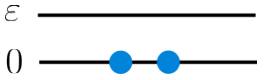
\includegraphics[width=0.25\linewidth]{Immagini/sistema a due livelli bosoni (i).png}
    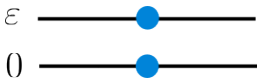
\includegraphics[width=0.25\linewidth]{Immagini/sistema a due livelli bosoni (ii).png}
    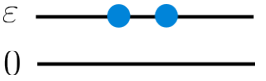
\includegraphics[width=0.25\linewidth]{Immagini/sistema a due livelli bosoni (iii).png}
    \caption{microstati: (i) $\ket{\nu}_1$; (i) $\ket{\nu}_2$; (i) $\ket{\nu}_3$.}
    \label{fig: sistema a due livelli bosoni}
\end{figure}
\paragraph{Fermioni.} Se le particelle sono fermioni, allora esiste un solo microstato possibile, mostrato in figura \ref{fig: sistema a due livelli fermioni}, dato da
\begin{equation}
    \ket{\nu} = \frac{1}{\sqrt{2!}}(\ket{1}_1 \otimes \ket{0}_2 + \ket{0}_1 \otimes \ket{1}_2).
\end{equation}
La funzione di partizione corrispondente è
\begin{equation}
    Z_F = \nsum_\nu e^{-\beta E_\nu} = e^{-\beta\epsilon}.
\end{equation}
\begin{figure}[h]
    \centering
    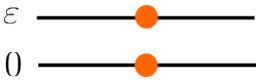
\includegraphics[width=0.25\linewidth]{Immagini/sistema a due livelli fermioni.png}
    \caption{l'unico microstato possibile per un sistema due livelli fermionico.}
    \label{fig: sistema a due livelli fermioni}
\end{figure}
\paragraph{Particelle distinguibili.} Per confronto, se si considerassero le particelle distinguibili, allora il numero di possibili microstati sarebbe quattro, mostrati in figura \ref{fig: sistema a due livelli classico}, e la funzione di partizione si fattorizzerebbe
\begin{equation}
    Z_D = |Z_{(1)}|^2 = (1 + e^{-\beta\epsilon})(1 + e^{-\beta\epsilon}) = 1 + 2e^{-\beta\epsilon} + e^{-2\beta\epsilon}.
\end{equation}
Confrontando $Z_D$ con $Z_B$ e $Z_F$, si nota come le interazioni statistiche non permettano alle funzioni di partizione bosonica e fermionica di fattorizzare; inoltre nel caso classico si era aggiunto il fattore di Gibbs per evitare l'omonimo paradosso, tuttavia se si segue questa strada si nota che
\begin{equation}
    Z_B \neq \frac{Z_D}{N!},\quad Z_F \neq \frac{Z_D}{N!}.
\end{equation}
\begin{figure}[h]
    \centering
    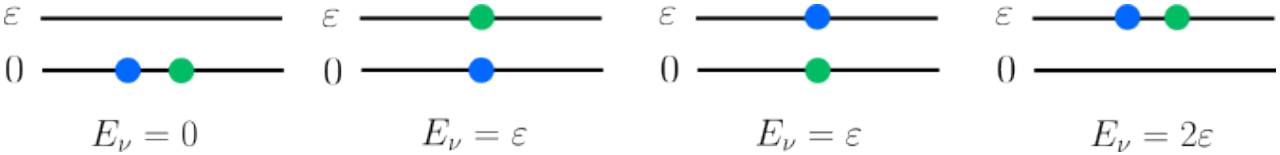
\includegraphics[width=0.95\linewidth]{Immagini/sistema a due livelli classico.png}
    \caption{possibili microstati per un sistema a due livelli classico.}
    \label{fig: sistema a due livelli classico}
\end{figure}
L'unico caso in cui vale l'uguaglianza le funzioni di partizione è quando le due particelle occupano livelli diversi. Dunque, il protocollo che si segue classicamente per evitare il paradosso di Gibbs è impreciso: vale solamente quando le componenti occupano tutte livelli differenti; tuttavia, nel caso del gas ideale, i livelli sono così densi che non succede praticamente mai che due particelle occupino lo stesso livello. 

\subsection{Coppia di particelle libere in una dimensione}
Si considerino due particelle in uno spazio unidimensionale con condizioni al contorno periodiche\footnote{Comunque, la generalizzazione tridimensionale, come anche l'inclusione delle condizioni di annullamento al bordo, non presenta particolari complicazioni.}. Per una singola particella, gli autostati di energia sono identificati da un numero
$m \in \Z$ con energia
\begin{equation}
    \epsilon_m = \frac{\hbar^2}{2m} \left( \frac{2\pi}{L} \right)^2 m^2,
\end{equation}
mentre per $N = 2$ particelle i possibili microstati bosonici $\ket{\nu_B}$ e fermionici $\ket{\nu_F}$ sono
identificati come 
\begin{equation}
\nu_B \longleftrightarrow \{ m_1 \ge m_2 \}, \quad
\nu_F \longleftrightarrow \{ m_1 > m_2 \}
\end{equation}
con energie
\begin{equation}
E_{\nu_B} = E_{\nu_F}
= \frac{\hbar^2}{2m} \left( \frac{2\pi}{L} \right)^2 (m_1^2 + m_2^2).
\end{equation}
Usando il fatto che
\begin{equation}
    \frac{\beta \pi^2}{2m} \left( \frac{2\pi}{L} \right)^2 = \frac{\pi \lambda_T^2}{L^2}
\end{equation}
la funzione di partizione bosonica risulta essere
\begin{equation}
    Z_B = \sum_{m_1 \ge m_2 \in \mathbb{Z}}e^{-\pi \lambda_T^2(m_1^2 + m_2^2)/L^2},
\end{equation}
dove la somma si può essere riorganizzata come
\begin{equation}
    \sum_{m_1 \ge m_2} = \frac{1}{2}
\bigg( \sum_{m_1, m_2} + \sum_{m_1 = m_2} \bigg),
\end{equation}
in questo modo l'espressione esatta della funzione di partizione bosonica diventa
\begin{equation}
    \begin{split}
        Z_B &= \frac{1}{2} \bigg( \sum_{m_1,m_2 \in \mathbb{Z}} e^{-\lambda_T^2(m_1^2+m_2^2)\pi/L^2} + \sum_{m \in \mathbb{Z}} e^{-2\lambda_T^2 m^2\pi/L^2} \bigg) \\
        &= \frac{1}{2} \bigg\{\bigg[\theta_3\bigg(\frac{i\lambda_T^2}{L^2}\bigg)\bigg]^2 + \theta_3\bigg(\frac{2i\lambda_T^2}{L^2}\bigg)\bigg\}.
    \end{split}
\end{equation}
Nel limite termodinamico $\lambda_T \ll L$ si ha
\begin{equation}
    Z_B = \frac{1}{2} \bigg[ \bigg( \frac{L}{\lambda_T} \bigg)^2 \left( 1 + 2 e^{-\pi L^2/\lambda_T^2} + \cdots \right) + \frac{L}{\sqrt{2}\lambda_T} \bigg( 1 + 2 e^{-\pi L^2/2\lambda_T^2} + \cdots \bigg) \bigg],
\end{equation}
ossia a meno di termini esponenzialmente soppressi
\begin{equation}
\label{eq: funzione di partizione bosonica sistema 2 particelle libere 1-dim}
    Z_B \simeq \frac{1}{2!} \bigg( \frac{L}{\lambda_T} \bigg)^2 \bigg( 1 + \frac{\lambda_T}{\sqrt{2}\,L} + \cdots \bigg),
\end{equation}
dove compaiono delle correzioni dovute ad interazioni statistiche create dall'indistinguibilità quantistica.
\begin{obs}
    Il risultato ottenuto nella \eqref{eq: funzione di partizione bosonica sistema 2 particelle libere 1-dim} è quello che si otterrebbe rimpiazzando le somme con integrali secondo
    \begin{equation}
        \frac{1}{2} \bigg( \sum_{m_1,m_2} + \sum_{m_1=m_2} \bigg) = \frac{1}{2}\bigg[\bigg( \frac{L}{2\pi} \bigg)^2 \int dk_1\, dk_2 + \frac{L}{2\pi} \int_{k_2=k_1} dk_1\bigg]
    \end{equation}
\end{obs}
Invece, la funzione di partizione fermionica è
\begin{equation}
    Z_F = \sum_{m_1>m_2} e^{-\lambda_T^2(m_1^2+m_2^2)/L^2},
\end{equation}
che sfruttando la riorganizzazione della somma seguente
\begin{equation}
    \sum_{m_1>m_2} = \frac{1}{2} \bigg( \sum_{m_1,m_2} - \sum_{m_2=m_1} \bigg)
\end{equation}
si procede con il conto esattamente come nel caso bosonico, arrivando all'espressione
\begin{equation}
\label{eq: funzione di partizione fermionica sistema 2 particelle libere 1-dim}
    Z_F = \frac{1}{2} \bigg\{\bigg[\theta_3\bigg(\frac{i\lambda_T^2}{L^2}\bigg)\bigg]^2 - \theta_3\bigg(\frac{2i\lambda_T^2}{L^2}\bigg)\bigg\} \simeq \frac{1}{2!} \bigg( \frac{L}{\lambda_T} \bigg)^2 \bigg( 1 - \frac{\lambda_T}{\sqrt{2}\,L} + \cdots \bigg)
\end{equation}

\subsection{Matrice densità}
Anche tramite il formalismo della matrice densità per i sistemi non interagenti emergono delle interazioni statistiche tra le componenti del sistema. Invece che rappresentare la matrice densità nella base dell'energia, in questo caso si sceglie la base delle posizioni; in ogni caso, la trattazione seguente è indipendente dalla scelta della base. Si indica quindi con $\{\ket{x}\}$ una base di stati della singola componente nella base degli autostati di posizione, per cui la funzione d'onda dello stato stazionario $\ket{a}$ è data da
\begin{equation}
    u_a(x) \equiv \mybraket{x}{a}.
\end{equation}
Per il sistema di $N$ componenti si indica la base degli autostati di posizione con
\begin{equation}
    \ket{x_1,\dots,x_N} = \ket{x_1}_1 \otimes \cdots \otimes \ket{x_N}_N.
\end{equation}
Se $\ket{\nu}$ è un stato stazionario, definito dalla \eqref{eq: microstato invariante per permutazioni}, la funzione d'onda $u_\nu$ associata è
\begin{equation}
    u_\nu \equiv \mybraket{x_1,\dots,x_N}{\nu} = \norm_\nu\nsum_P\delta_P\mybraket{x_1}{a_{P(1)}}\cdots\mybraket{x_N}{a_{P(N)}},
\end{equation}
dove il fattore di normalizzazione $\norm_\nu$ è sempre dato dalla \eqref{eq: normalizzazione microstati sistemi non interagenti identici}. Considerando che
\begin{equation}
\label{eq: proprietà produttoria}
    \nprod_if(i) = \nprod_if[P^{-1}(i)]
\end{equation}
dato che la permutazione riarrangia solamente l'ordine dei fattori, si può riscrivere $u_\nu$ tenendo fissi gli stati $\ket{a_i}$ e permutando le $x_i$, così da avere
\begin{equation}
    u_\nu = \norm_\nu\nsum_{P^{-1}}\delta_{P^{-1}}\mybraket{x_{P^{-1}(1)}}{a_1}\cdots\mybraket{x_{P^{-1}(N)}}{a_N}.
\end{equation}
Considerando che sommare su tutte le permutazioni $P$ o sugli inversi delle permutazioni $P^{-1}$ è equivalente, per cui
\begin{equation}
    \nsum_P \equiv \nsum_{P^{-1}},\quad \delta_P = \delta_{P^{-1}}
\end{equation}
è quindi possibile scrivere 
\begin{equation}
\label{eq: funzione onda sistemi non interagente identico}
    \begin{split}
        u_\nu &= \norm_\nu\nsum_P\delta_P\mybraket{x_{P(1)}}{a_1}\cdots\mybraket{x_{P(N)}}{a_N} \\
        &= \norm_\nu\nsum_P\delta_Pu_{a_1}[x_{P(1)}]\cdots u_{a_N}[x_{P(N)}].
    \end{split}
\end{equation}
Quindi, la matrice densità canonica è data da
\begin{equation}
    \rho(x_1,\dots,x_N;y_1,\dots,y_N) = \mybrakett{x_1,\dots,x_N}{\frac{e^{-\beta\hatH}}{Z}}{y_1,\dots,y_N}.
\end{equation}
Inserendo una relazione di completezza $\nsum_\nu\ket{\nu}\bra{\nu} = \MI$ nella definizione di $\rho(x_i;y_i) \equiv \rho(x_1,\dots,x_N;y_1,\dots,y_N)$, segue che 
\begin{equation}
    \begin{split}
        \rho(x_i;y_i) &= \frac{1}{Z}\nsum_\nu\mybraket{x_1,\dots,x_N}{\nu}\mybraket{\nu}{y_1,\dots,y_N}e^{-\beta E_\nu} \\
        &= \frac{1}{Z}\nsum_\nu u_\nu^*(y_1,,\dots,y_N)u_{\nu}(x_1,\dots,x_N)e^{-\beta E_\nu} \\
        &= \frac{1}{Z}\nsum_\nu|\norm_\nu|^2\nsum_{P,Q}\delta_P\delta_Qu_{a_1}^*[y_{P(1)}]u_{a_1}[x_{Q(1)}]\\
        &\times\cdots\times u_{a_N}^*[y_{P(N)}]u_{a_N}[x_{Q(N)}]e^{-\beta(\epsilon_{a_1}+\cdots+\epsilon_{a_N})} \\
        &= \frac{1}{Z}\nsum_\nu|\norm_\nu|^2\nsum_{P,Q}\delta_P\delta_Qu_{a_1}^*[y_{PQ^{-1}(1)}]u_{a_1}(x_1)\\
        &\times\cdots\times u_{a_N}^*[y_{PQ^{-1}(N)}]u_{a_N}(x_N)e^{-\beta(\epsilon_{a_1}+\cdots+\epsilon_{a_N})},
    \end{split}
\end{equation}
dove nel penultimo e nell'ultimo passaggio si sono usate rispettivamente le equazioni \eqref{eq: funzione onda sistemi non interagente identico} e \eqref{eq: proprietà produttoria}. Dato che una delle permutazioni è ridondante si riduce ad un fattore $N!$, inoltre ponendo $R \equiv PQ^{-1}$ si ha $\delta_P\delta_Q = \delta_P\delta_{Q^{-1}} \equiv \delta_R$ e mappando la somma sui microstati con quella che conta sugli stati $a_i$ ordinati, per cui si ottiene
\begin{equation}
    \begin{split}
        \rho(x_i,y_i) = \frac{1}{Z}\nsum_\nu|\norm_\nu|^2\nsum_Pf(\{a_i\}) &= \frac{N!}{Z}\nsum_\nu|\norm_\nu|^2f(\{a_i\}) \\
        &= \frac{1}{Z}\sum_{a_1\ge\cdots\ge a_N}\frac{f(\{a_i\})}{\nprod_a n_a!},
    \end{split}
\end{equation}
dove si sostituita l'espressione del fattore di normalizzazione \eqref{eq: normalizzazione microstati sistemi non interagenti identici} e si è posta la funzione $f(\{a_i\})$ del microstato invariante (a meno di un segno globale nel caso fermionico) per permutazioni delle $a_i$ come
\begin{equation}
    f(\{a_i\}) \equiv \nsum_{R}\delta_Ru_{a_1}^*[y_{R(1)}]u_{a_1}(x_1)\cdots u_{a_N}^*[y_{R(N)}]u_{a_N}(x_N)e^{-\beta(\epsilon_1+\cdots+\epsilon_N)};
\end{equation}
inoltre, notando che la sommatoria ordinata si può scrivere senza vincoli sull'ordinamento stesso, in termini della somma indipendente su tutti gli stati $a_i$ si ha
\begin{equation}
    \begin{split}
        \rho(x_i,y_i) &= \frac{1}{N!Z}\sum_{a_1,\cdots,a_N}f(\{a_i\}) \\
        &= \frac{1}{N!Z}\sum_{a_1,\cdots,a_N}\nsum_{R}\delta_Ru_{a_1}^*[y_{R(1)}]u_{a_1}(x_1)\\
        &\times\cdots\times u_{a_N}^*[y_{R(N)}]u_{a_N}(x_N)e^{-\beta(\epsilon_1+\cdots+\epsilon_N)} \\
        &= \frac{1}{N!Z}\nsum_{R}\delta_R\nsum_{a_1}u_{a_1}^*[y_{R(1)}]u_{a_1}(x_1)e^{-\beta\epsilon_{a_1}}\\
        &\times\cdots\times\nsum_{a_N}u_{a_N}^*[y_{R(N)}]u_{a_N}(x_N)e^{-\beta\epsilon_N},
    \end{split}
\end{equation}
da cui in definitiva, riconoscendo in ogni somma indipendente sugli stati $a_i$ le matrici densità di singola particella mancanti della normalizzazione $1/Z_{(1)}$, si ottiene
\begin{equation}
\label{eq: matrice densità sistemi non interagenti identici}
    \rho(x_1,\dots,x_N;y_1,\dots,y_N) = \frac{[Z_{(1)}]^N}{N!Z}\nsum_R\delta_R\rho[x_1,y_{R(1)}]\cdots\rho[x_N,y_{R(N)}].
\end{equation}
La statistica entra in gioco ``mescolando'' i termini. L'equazione \eqref{eq: matrice densità sistemi non interagenti identici} mostra come siano presenti delle ``interazioni statistiche'' tra le varie componenti pur non avendo termini di interazioni nell'hamiltoniana del sistema in quanto la matrice densità non è fattorizzata nelle varie componenti. 

\subsection{\texorpdfstring{$N$}{N} particelle libere in tre dimensioni}
Sfruttando il formalismo della matrice densità, in questo caso si ha
\begin{equation}
    \rho(\vx_i,\vx_j) = \frac{1}{V}\exp{\bigg(-\frac{\prod_{i,j}|\vx_i - \vx_j|^2}{\lambda_T^2}\bigg)} \equiv \frac{f_{ij}}{V}.
\end{equation}
Usando la relazione \eqref{eq: funzione di partizione singola particella (canonico)} per la funzione di partizione di singola particelle $Z_{(1)}$ si può scrivere
\begin{equation}
\label{eq: matrice densità sistemi non interagenti identici N particelle 3-dim}
    \begin{split}
        Z\rho(\vx_i,\vx_j) &= \frac{1}{N!}\bigg(\frac{V}{V_T}\bigg)^N\nsum_P\delta_P\frac{f_{1,P(1)}}{V}\cdots\frac{f_{N,P(N)}}{V} \\
        &= \frac{1}{V_T^NN!}\nsum_P\delta_Pf_{1,P(1)}\cdots f_{N,P(N)}.
    \end{split}
\end{equation}
Si nota che per i termini diagonali della matrice densità, i quali codificano la probabilità di trovare il sistema con determinate posizioni, si ha $f_{ii} = 1$; quindi, per ogni permutazione $P$ nella somma a secondo membro della \eqref{eq: matrice densità sistemi non interagenti identici N particelle 3-dim} ogni coordinata lasciata invariata da $P$ contribuisce con un fattore pari a $1$. Pertanto, si ha un termine non banale solo per le coordinate che vengono permutate. Integrando la \eqref{eq: matrice densità sistemi non interagenti identici N particelle 3-dim} sulle coordinate $\vx_1,\dots,\vx_N$ si ottiene la funzione di partizione $Z$ dato che la matrice densità è normalizzata ad uno per costruzione. Dunque, si ha
\begin{equation}
\label{eq: funzione di partizione sistemi non interagenti identici N particelle 3-dim}
    Z = \frac{1}{V_T^NN!}\nsum_P\delta_P\int d^3x_1\cdots d^3x_N\,f_{1,P(1)}\cdots f_{N,P(N)}.
\end{equation}
Nella funzione di partizione \eqref{eq: funzione di partizione sistemi non interagenti identici N particelle 3-dim} le variabili $\vx_i$ sono integrate, ossia mute, per cui l'etichetta delle $x$ non è rilevante: se si riordinassero le $\vx$ tra di loro non cambierebbe nulla; in altre parole, tutte le permutazioni appartenenti alla stessa classe di coniugazione ($[P] = \{Q^{-1}PQ\},\,Q\in S_n$) restituiscono lo stesso contributo. 
\paragraph{Classe dell'identità.} La classe di coniugazione dell'identità contiene solo l'identità
\begin{equation}
    P = \MI \to \int d^3x_1\cdots d^3x_N\,f_{1,1}\cdots f_{N,N} = \int d^3x_1\cdots d^3x_N = V^N.
\end{equation}
\paragraph{Classe degli scambi $i\leftrightarrow j$.} La classe di coniugazione degli scambi contiene le permutazioni $P$ che lasciano fissi $(N-2)$ elementi e
ne scambiano due fra di loro. Quindi, nell'integrale si hanno $f_{12}$, $f_{21}$ e da $f_{33}$ in poi si hanno tutti termini uguali pari ad $1$. Per queste permutazioni $\delta_P = \pm 1$ per bosoni o fermioni rispettivamente. Dunque, il numero di scambi è $\binom{N}{2}$, corrispondente alla scelta degli elementi scambiati. 
\begin{ex}
    Per lo scambio $(1 \leftrightarrow 2)$ si ottiene
    \begin{multline}
    \label{eq: permutazione scambio 1 - 2}
        \int d^3 x_1 d^3 x_2\,f_{12} f_{21} \int d^3 x_3 \cdots d^3 x_N\,1 \cdot 1 \cdots =\\
        = V^{N-2} \int d^3 x_1 \int d^3 x_2\,\exp\bigg[{- \frac{\pi}{\lambda_T^2} (|\vx_{12}|^2 + |\vx_{21}|^2)}\bigg],
    \end{multline}
    dove $|\vx_{12}|^2 + |\vx_{21}|^2
        = 2\, |\vx_{12}|^2$. Ora, con il cambio di variabili dato da
    \begin{equation}
        \begin{cases}
            \vx_{CM} = \dfrac{1}{2}(\vx_1 + \vx_2) \\[2ex]
        \vz \equiv \vx_{12} = \vx_1 - \vx_2
        \end{cases}
    \end{equation}
    avente jacobiano pari a $1$, la \eqref{eq: permutazione scambio 1 - 2} diventa
    \begin{equation}
        V^{N-2} \int d^3 x_{CM} \int d^3 z \, \exp{\bigg(-\frac{2\pi}{\lambda_T^2}|z|^2\bigg)} = V^{N-2} V \bigg( \frac{\lambda_T^2}{2} \bigg)^{3/2} =  \frac{V_T}{V} \frac{V^N}{2^{3/2}}
    \end{equation}
\end{ex}

\subsubsection{Limite di alta temperatura}
Nel limite di alta temperatura per cui $V_T \ll V$, le classi di permutazioni che contengono più di uno scambio sono ulteriormente soppresse in quanto contengono potenze più alte di $V_T/V$. Dunque, si può ridurre la funzione di partizione \eqref{eq: funzione di partizione sistemi non interagenti identici N particelle 3-dim} all'espressione
\begin{equation}
    Z = \frac{1}{N!}\bigg(\frac{V}{V_T}\bigg)^N\bigg[1 + \binom{N}{2}\frac{V_T}{2^{3/2}V} + \cdots \bigg],
\end{equation}
la quale rappresenta una generalizzazione per un sistema di $N$ particelle in uno spazio tridimensionale delle funzioni di partizione bosonica \eqref{eq: funzione di partizione bosonica sistema 2 particelle libere 1-dim} e fermionica \eqref{eq: funzione di partizione fermionica sistema 2 particelle libere 1-dim}. La coda di correzioni dovute alle permutazioni non banali, soppresse dal limite di alta temperatura $V_T/V$, sono, come già detto, un effetto di interazione di natura statistica. Queste interazioni possono diventare significative e dare luogo a comportamenti non banali di $Z$, e quindi delle grandezze termodinamiche, nel regime di bassa temperatura in cui $V_T$ diviene comparabile o superiore a $V$.

\subsubsection{Considerazioni}
Riassumendo quanto fatto, il modo più immediato per scrivere la funzione di partizione nell'ensemble canonico consiste nel caratterizzare gli stati tramite il formalismo dei numeri di occupazione, in particolare
\begin{equation}
    \ket{\nu} \longleftrightarrow \{n_a\} : \nsum_a n_a = N,\quad n_a \in 
    \begin{cases}
        \N_0\,\mathrm{bosoni} \\
        \{0,1\} \,\mathrm{fermioni}
    \end{cases},
\end{equation}
in termini dei quali l'energia dei microstati è $E_\nu = \nsum_a n_a\epsilon_a$, risultando quindi in una funzione di partizione della forma
\begin{equation}
    Z= \nsum_\nu e^{-\beta E_\nu} = \nsum_{\{n_a\}}e^{-\beta\nsum_an_a\epsilon_a}.
\end{equation}
Per un generico sistema con $N$ elevato, la presenza del vincolo $\nsum_a n_a = N$ nella sommatoria rende complesso determinare $Z$. Sarebbe più semplice se si potesse fare una somma indipendente: se si sommasse su $n_a$ senza avere il vincolo su $N$, si otterrebbe un sistema aperto. Per questa ragione, risulta conveniente trattare i gas ideali quantistici nell'ensemble grancanonico.